\documentclass[12pt, letterpaper]{report}

% ==========================================================
%  PAQUETE PERSONALIZADO (Carga todas las normas ICONTEC)
% ==========================================================
\usepackage{icontec}

% --- BIBLIOGRAFÍA ---
\addbibresource{IFSA.bib}
\usepackage{csquotes}
% ==========================================================
%  PAQUETES COMPLEMENTARIOS (Matematicas, Graficos, Codigo)
% ==========================================================
% --- MATEMATICAS ---
\usepackage{amsmath,amssymb,amsthm}
\usepackage{mathtools}
\usepackage{braket}
\usepackage{bm}

% --- GRAFICOS Y PLOTS ---
\usepackage{graphicx}
\graphicspath{{../imagenes/}}
\usepackage{tikz}
\usetikzlibrary{
    3d, calc, intersections, perspective, arrows,
    arrows.meta, babel, decorations.markings, patterns,
    shapes.geometric, positioning, fadings, decorations.pathreplacing
}
\usepackage{float}
\usepackage{array}
\usepackage{pgfplots}
\pgfplotsset{compat=1.17}

% --- CODIGO FUENTE  ---
\usepackage{listings}
\usepackage{xcolor}

\definecolor{codegreen}{rgb}{0.11,0.35,0.02}
\definecolor{codegray}{rgb}{0.5,0.5,0.5}
\definecolor{codepurple}{rgb}{0.58,0,0.82}
\definecolor{backcolour}{rgb}{0.96,0.96,0.96}

\lstdefinestyle{FreeFEM}{
    backgroundcolor=\color{backcolour},
    commentstyle=\color{codegreen},
    keywordstyle=\color{blue}\bfseries,
    numberstyle=\tiny\color{codegray},
    stringstyle=\color{codepurple},
    basicstyle=\ttfamily\small,
    breaklines=true,
    captionpos=b,
    keepspaces=true,
    numbers=left,
    numbersep=5pt,
    showstringspaces=false,
    tabsize=4,
    frame=Ltb,
    inputencoding=utf8,
    extendedchars=true,
    literate={á}{{\'a}}1 {é}{{\'e}}1 {í}{{\'i}}1 {ó}{{\'o}}1 {ú}{{\'u}}1 
    {Á}{{\'A}}1 {É}{{\'E}}1 {Í}{{\'I}}1 {Ó}{{\'O}}1 {Ú}{{\'U}}1 
    {ñ}{{\~n}}1 {Ñ}{{\~N}}1 {ü}{{\"u}}1 {Ü}{{\"U}}1,
}
\lstset{style=FreeFEM}

% --- HIPERVINCULOS ---
\usepackage[colorlinks=true, linkcolor=blue, citecolor=blue, urlcolor=blue]{hyperref}

% --- ENTORNOS TIPO TEOREMA ---
\theoremstyle{definition}
\newtheorem{teorema}{Teorema}[chapter]
\newtheorem{corolario}{Corolario}[chapter]
\newtheorem{lema}{Lema}[chapter]
\newtheorem{definicion}{Definición}[chapter]
\newtheorem{ejemplo}{Ejemplo}[chapter]
\newtheorem*{nota}{Nota}

% ==========================================================
%  DATOS DEL DOCUMENTO
% ==========================================================
\newcommand{\titulo}{DESCRIPCIÓN Y SIMULACIÓN DE UN MODELO MATEMÁTICO PARA PROBLEMAS ACOPLADOS FLUIDO-ESTRUCTURA USANDO EL MÉTODO DE ELEMENTOS FINITOS}
\newcommand{\nombreestudiante}{SHARON NICOLE ACOSTA CARABALLO}
\newcommand{\nombredirector}{HUMBERTO PEREZ GONZALEZ}
\newcommand{\titulodirector}{PhD}
\newcommand{\fecha}{2026}

% ==========================================================
%  CUERPO DEL DOCUMENTO
% ==========================================================
\begin{document}

% --- PORTADA ---
\begin{titlepage}
    \centering
    \begin{singlespace}
        {\large\bfseries UNIVERSIDAD DE CARTAGENA\par}
        \vspace{0.5cm}
        
\includegraphics[width=40mm]{udc.png}\par
        \vfill
        {\Large\bfseries \titulo\par}
        \vfill
        {\large\bfseries \nombreestudiante\par}
        \vfill
        {\small Trabajo de grado para optar al título de Matemático\par}
        \vfill
        \textbf{Director:}\par
        {\large \nombredirector, \titulodirector\par}
        \vfill
        {\large FACULTAD DE CIENCIAS EXACTAS Y NATURALES\par
        PROGRAMA DE MATEMÁTICAS\par
        CARTAGENA DE INDIAS\par}
        \fecha
    \end{singlespace}
\end{titlepage}

% --- PRELIMINARES ---
\pagenumbering{roman}
\tableofcontents
\listoffigures
\listoftables
\newpage

% --- CONTENIDO PRINCIPAL ---
\pagenumbering{arabic} 



\chapter*{Introducción}
\addcontentsline{toc}{chapter}{Introducción}



El estudio de los fenómenos multifísicos representa uno de los campos más dinámicos e interdisciplinarios de la matemática aplicada moderna. Entre estos fenómenos, los problemas acoplados de Interacción Fluido-Estructura (FSI, por sus siglas en inglés) ocupan un lugar preeminente debido a su complejidad intrínseca y a su ubicuidad en la naturaleza y la industria. Tradicionalmente, la dinámica de fluidos y la mecánica de sólidos elásticos se han abordado de forma aislada mediante el análisis de los sistemas diferenciales de Stokes o Navier-Stokes y de la elasticidad lineal de Lamé, respectivamente. Sin embargo, en escenarios reales, ambos medios coexisten e interactúan dinámicamente en una interfaz común: el flujo ejerce fuerzas hidrodinámicas que deforman la estructura, y dicha deformación modifica sustancialmente el dominio geométrico en el que se desplaza el fluido, dando lugar a un acoplamiento bidireccional fuertemente no lineal.

Desde la perspectiva de un profesional en matemáticas, el interés fundamental de este trabajo de grado no radica únicamente en la ejecución computacional de un simulador numérico, sino en el riguroso puente conceptual construido entre el análisis funcional abstracto y la computación científica. La transición desde las ecuaciones diferenciales parciales en su forma fuerte hacia sus contrapartes variacionales exige un estudio pormenorizado de los espacios de Sobolev ($L^2$, $H^1$ y $H_0^1$) y de operadores bilineales, garantizando la existencia y unicidad de las soluciones mediante el Teorema de Lax-Milgram. Aceptando este marco teórico, el propósito medular de esta investigación consistió en describir, analizar e implementar de forma consistente las condiciones cinemáticas y dinámicas de acoplamiento que gobiernan dicha interfaz móvil, evaluando el impacto de la discretización espacial en la estabilidad global del sistema.

Para dar cumplimiento a este propósito y validar la consistencia de los modelos estudiados, el presente trabajo se estructuró bajo una ruta metodológica y matemática precisa. En primer lugar, se fundamentaron los conceptos analíticos esenciales del Método de los Elementos Finitos (FEM) y la formulación de Galerkin, examinando el comportamiento del error mediante herramientas clásicas como el Lema de Céa y el argumento de dualidad de Aubin-Nitsche. Posteriormente, se dedujeron y acoplaron las ecuaciones diferenciales que gobiernan el fluido viscoso y la estructura elástica, formulando el problema variacional global y su estrategia de resolución mediante un esquema numérico particionado iterativo con relajación.

Finalmente, el modelo matemático integral se codificó y ejecutó en la plataforma de cálculo científico FreeFEM++, tomando como caso de estudio el problema benchmark de una cavidad vertical sujeta a un flujo inducido y sellada en su parte superior por una viga elástica deformable. Esta aproximación computacional permitió examinar el comportamiento geométrico del dominio deformado mediante la técnica Arbitraria Lagrangiana-Euleriana (ALE) y, como complemento al análisis teórico, estimar experimentalmente la tasa de convergencia del error mediante refinamiento de mallas ($h$-refinement). Así, este documento expone cómo las herramientas abstractas del análisis moderno se consolidan como el cimiento indispensable para la resolución numérica de problemas multifísicos complejos.


El cuerpo de este trabajo de grado se encuentra organizado de la siguiente manera:

El \textbf{Capítulo 1} sienta las bases del método de los elementos finitos, abordando los espacios funcionales necesarios, la derivación detallada de la forma débil, la aproximación a través del método de Galerkin y las estimaciones formales de error. En el \textbf{Capítulo 2}, se profundiza en la formulación fuerte y débil de los dos subproblemas independientes, describiendo analíticamente la física del fluido viscoso mediante las ecuaciones de Stokes y la deformación del sólido a través de las ecuaciones de la elasticidad lineal. Ese mismo \textbf{Capítulo 2} constituye el núcleo de la investigación: en él se explican las condiciones de transmisión cinemática y dinámica en la interfaz, la formulación variacional del problema acoplado y la estrategia numérica particionada empleada para resolverlo. El \textbf{Capítulo 3} expone la implementación computacional en FreeFEM++, detallando la configuración geométrica de la cavidad con tapa elástica, la técnica Arbitraria Lagrangiana-Euleriana (ALE) para el movimiento de malla, las simulaciones obtenidas y el análisis de convergencia numérica. Por último, el \textbf{Capítulo 4} discute de manera crítica los alcances y limitaciones del modelo y recoge las conclusiones y las líneas de trabajo futuro.

% CAPÍTULO 1: TEORÍA
\chapter{Fundamentos del método de elementos finitos}
\label{chap:teoria}

\section{Introducción al método de los elementos finitos}

El método de los elementos finitos (MEF) constituye una herramienta numérica fundamental para la resolución aproximada de ecuaciones en derivadas parciales (EDP) en dominios complejos. Su versatilidad lo convierte en el estándar para la modelización de fenómenos multifísicos, como la interacción fluido-estructura abordada en este trabajo \cite{hou2012numerical, bungartz2006fluid, kolahdouz2023sharp}. En particular, se adopta el enfoque de Galerkin, el cual demuestra una alta efectividad para problemas de equilibrio y flujo viscoso estacionario \cite{quarteroni2008numerical}.

La aplicación de este método se estructura sobre tres pilares teóricos fundamentales:

\begin{enumerate}
    \item \textbf{Formulación débil:} Consiste en la transformación del problema diferencial fuerte a una forma integral o variacional. Este procedimiento no solo reduce los requisitos de regularidad (suavidad) de la solución, sino que permite incorporar las condiciones de frontera de tipo Neumann de manera natural, aspecto fundamental para el acoplamiento de tensiones en la interfaz fluido-sólido.
    
    \item \textbf{Discretización del dominio:} Implica la partición del dominio continuo $\Omega$ en un conjunto de subdominios elementales (malla), denotada como $\mathcal{T}_h$. Esta discretización posibilita la aproximación precisa de la geometría de la cavidad, incluso cuando esta se deforma por la acción del fluido.
    
    \item \textbf{Aproximación por subespacios:} Se basa en la construcción de espacios de dimensión finita $V_h$ mediante funciones base polinómicas a trozos definidas sobre la malla. Esto transforma el problema variacional continuo en un sistema algebraico de ecuaciones lineales, el cual es resoluble computacionalmente de manera eficiente \cite{hecht2012new}.
\end{enumerate}

En las secciones subsiguientes se desarrollará la formulación matemática específica para el sistema acoplado Stokes-Elasticidad, detallando la elección de los espacios de elementos finitos necesarios para garantizar la estabilidad numérica y la convergencia de la solución.

\section{Formulación matemática del método de los elementos finitos}

El método de los elementos finitos (MEF) se fundamenta en la formulación variacional o débil de las ecuaciones en derivadas parciales. A diferencia de la formulación clásica (o fuerte), que exige una alta regularidad en la solución (típicamente de clase $C^2$), la formulación débil permite buscar soluciones en espacios funcionales más generales, conocidos como espacios de Sobolev \cite{quarteroni2008numerical}.

\subsection{Espacios funcionales y notación}

Sea $\Omega \subset \mathbb{R}^d$ (con $d=1, 2, 3$) un dominio acotado con frontera Lipschitz $\Gamma = \partial \Omega$. Se denota por $L^2(\Omega)$ el espacio de funciones de cuadrado integrable sobre $\Omega$, dotado del producto interno:
\[
(u, v)_{0,\Omega} = \int_{\Omega} u(\mathbf{x}) v(\mathbf{x}) \, d\mathbf{x},
\]
y la norma asociada $\|u\|_{0,\Omega} = (u, u)_{0,\Omega}^{1/2}$.

Para formular problemas de segundo orden, se introduce el espacio de Sobolev $H^1(\Omega)$, definido como:
\[
H^1(\Omega) = \left\{ v \in L^2(\Omega) : \frac{\partial v}{\partial x_i} \in L^2(\Omega), \quad \forall i=1,\dots,d \right\},
\]
donde las derivadas se entienden en el sentido de las distribuciones. La norma en este espacio está dada por:
\[
\|v\|_{1,\Omega} = \left( \|v\|_{0,\Omega}^2 + \sum_{i=1}^d \left\| \frac{\partial v}{\partial x_i} \right\|_{0,\Omega}^2 \right)^{1/2}.
\]
Para problemas con condiciones de frontera de Dirichlet homogéneas, se define el subespacio $H^1_0(\Omega)$, el cual consiste en las funciones de $H^1(\Omega)$ que se anulan en la frontera $\Gamma$ en el sentido de la traza \cite{adams2003sobolev}:
\[
H^1_0(\Omega) = \{ v \in H^1(\Omega) : v|_{\Gamma} = 0 \}.
\]

\subsection{Derivación de la forma débil}

Considérese el problema modelo de Poisson con condiciones de Dirichlet homogéneas:
\begin{equation}\label{eq:poisson_fuerte}
    \begin{aligned}
        -\nabla \cdot (\kappa \nabla u) &= f \quad \text{en } \Omega, \\
        u &= 0 \quad \text{sobre } \Gamma,
    \end{aligned}
\end{equation}
donde $\kappa = \kappa(\mathbf{x})$ es un coeficiente de difusión positivo y acotado, y $f \in L^2(\Omega)$.

Para obtener la formulación débil, se multiplica la ecuación \eqref{eq:poisson_fuerte} por una función de prueba arbitraria $v \in H^1_0(\Omega)$ y se integra sobre el dominio $\Omega$:
\[
-\int_{\Omega} \nabla \cdot (\kappa \nabla u) v \, d\mathbf{x} = \int_{\Omega} f v \, d\mathbf{x}.
\]
Aplicando la primera identidad de Green (consecuencia del teorema de la divergencia):
\[
\int_{\Omega} \kappa \nabla u \cdot \nabla v \, d\mathbf{x} - \int_{\Gamma} \kappa (\nabla u \cdot \mathbf{n}) v \, ds = \int_{\Omega} f v \, d\mathbf{x},
\]
donde $\mathbf{n}$ es el vector normal unitario exterior a $\Gamma$. Dado que $v \in H^1_0(\Omega)$, se tiene que $v = 0$ sobre $\Gamma$, por lo que la integral de frontera se anula. Así, se llega al problema variacional abstracto:

\begin{definicion}[Problema variacional]
    Hallar $u \in V$ tal que:
    \begin{equation}\label{eq:problema_variacional}
        a(u, v) = L(v), \quad \forall v \in V,
    \end{equation}
    donde $V = H^1_0(\Omega)$, y las formas bilineal $a(\cdot,\cdot)$ y lineal $L(\cdot)$ se definen como:
    \[
    a(u, v) = \int_{\Omega} \kappa \nabla u \cdot \nabla v \, d\mathbf{x}, \quad L(v) = \int_{\Omega} f v \, d\mathbf{x}.
    \]
\end{definicion}

La equivalencia entre la forma fuerte \eqref{eq:poisson_fuerte} y la forma débil \eqref{eq:problema_variacional} se establece en el sentido de las distribuciones.

\subsubsection*{Formulación en componentes escalares}

En un dominio bidimensional $\Omega \subset \mathbb{R}^2$ con coordenadas cartesianas $(x,y)$, el sistema fuerte \eqref{eq:poisson_fuerte} puede expresarse de forma explícita mediante la suma de sus derivadas parciales:

\begin{equation} \label{eq:poisson_fuerte_escalar}
    -\left[ \frac{\partial}{\partial x} \left( \kappa \frac{\partial u}{\partial x} \right) + \frac{\partial}{\partial y} \left( \kappa \frac{\partial u}{\partial y} \right) \right] = f(x,y).
\end{equation}

Para obtener la forma débil, se multiplica la ecuación anterior por la función de prueba $v(x,y)$ y se integra sobre el dominio:

\begin{equation}
    -\int_{\Omega} \frac{\partial}{\partial x} \left( \kappa \frac{\partial u}{\partial x} \right) v \, dx dy - \int_{\Omega} \frac{\partial}{\partial y} \left( \kappa \frac{\partial u}{\partial y} \right) v \, dx dy = \int_{\Omega} f v \, dx dy.
\end{equation}

Al aplicar integración por partes en cada término de forma independiente, se tiene:

\begin{itemize}
    \item Para la dirección $x$: 
    \[ -\int_{\Omega} \frac{\partial}{\partial x} \left( \kappa \frac{\partial u}{\partial x} \right) v \, d\Omega = \int_{\Omega} \kappa \frac{\partial u}{\partial x} \frac{\partial v}{\partial x} \, d\Omega - \int_{\Gamma} \kappa \frac{\partial u}{\partial x} v n_x \, d\Gamma. \]
    \item Para la dirección $y$: 
    \[ -\int_{\Omega} \frac{\partial}{\partial y} \left( \kappa \frac{\partial u}{\partial y} \right) v \, d\Omega = \int_{\Omega} \kappa \frac{\partial u}{\partial y} \frac{\partial v}{\partial y} \, d\Omega - \int_{\Gamma} \kappa \frac{\partial u}{\partial y} v n_y \, d\Gamma. \]
\end{itemize}

Sumando ambas ecuaciones y considerando que $v=0$ sobre la frontera $\Gamma$, se obtiene la forma variacional expandida:

\begin{equation}
    \int_{\Omega} \kappa \left( \frac{\partial u}{\partial x} \frac{\partial v}{\partial x} + \frac{\partial u}{\partial y} \frac{\partial v}{\partial y} \right) d\Omega = \int_{\Omega} f v \, d\Omega.
\end{equation}

Esta expresión permite identificar que la forma bilineal $a(u,v)$ es el resultado de sumar las contribuciones de la difusión en cada eje coordenado, facilitando la construcción de las matrices elementales en el método de los elementos finitos.

\subsection*{Construcción genérica de la forma débil para sistemas vectoriales}

Cuando la incógnita es un campo vectorial $\mathbf{u} = (u_1, u_2, \dots, u_d)$, el problema fuerte se compone de un sistema de $d$ ecuaciones diferenciales acopladas. El procedimiento para obtener su forma débil en componentes sigue estos pasos:

\subsubsection*{1. Identificación de las ecuaciones del sistema}
Cada componente $i$ del sistema fuerte satisface una ecuación de equilibrio. De forma genérica, para $i = 1, \dots, d$:
\begin{equation}
    -\sum_{j=1}^d \mathcal{L}_{ij}(u_j) = f_i \quad \text{en } \Omega
\end{equation}
donde $\mathcal{L}_{ij}$ es el operador que relaciona la componente $u_j$ con la $i$-ésima ecuación.

\subsubsection*{2. Multiplicación por funciones de prueba y suma}
Introducimos un vector de funciones de prueba $\mathbf{v} = (v_1, v_2, \dots, v_d)$. Multiplicamos cada ecuación $i$ por su correspondiente componente $v_i$ e integramos la suma de todas ellas sobre el dominio $\Omega$:
\begin{equation}
    \sum_{i=1}^d \left( \int_{\Omega} \left[ -\sum_{j=1}^d \mathcal{L}_{ij}(u_j) \right] v_i \, d\Omega \right) = \sum_{i=1}^d \int_{\Omega} f_i v_i \, d\Omega.
\end{equation}

\subsubsection*{3. Integración por partes y acoplamiento}
Aplicando el teorema de la divergencia (o integración por partes) a los términos de orden superior, distribuimos las derivadas entre las incógnitas $u_j$ y las funciones de prueba $v_i$. La forma bilineal resultante $a(\mathbf{u}, \mathbf{v})$ se visualiza como:
\begin{equation}
    a(\mathbf{u}, \mathbf{v}) = \sum_{i=1}^d \sum_{j=1}^d \int_{\Omega} \mathcal{A}_{ij}(u_j, v_i) \, d\Omega.
\end{equation}

\subsubsection*{4. Interpretación para la implementación (Matrices de bloques)}
Esta estructura en componentes es la que dicta la formación de la matriz de rigidez global $\mathbf{K}$ en el método de elementos finitos:
\begin{itemize}
    \item Los términos donde $i=j$ generan los \textbf{bloques diagonales} $\mathbf{K}_{ii}$, que representan la auto-influencia de cada componente.
    \item Los términos donde $i \neq j$ generan los \textbf{bloques de acoplamiento} $\mathbf{K}_{ij}$, que describen cómo la componente $j$ afecta a la ecuación de la dirección $i$.
\end{itemize}

De este modo, el problema variacional consiste en hallar el vector $\mathbf{u} \in \mathbf{V}$ tal que la suma de todas las contribuciones internas sea igual a la suma de los trabajos externos para cualquier vector de prueba $\mathbf{v} \in \mathbf{V}$.

\subsubsection{Existencia y unicidad de la solución}

El buen planteamiento del problema variacional (existencia y unicidad de solución) se garantiza mediante el teorema de Lax-Milgram \cite{ciarlet2002finite}.

\begin{teorema}[Lax-Milgram]
    Sea $V$ un espacio de Hilbert real con norma $\|\cdot\|_V$. Sea $a: V \times V \to \mathbb{R}$ una forma bilineal y $L: V \to \mathbb{R}$ un funcional lineal. Si se cumplen las siguientes condiciones:
    \begin{enumerate}
        \item \textbf{Continuidad de $a$:} Existe $M > 0$ tal que $|a(u, v)| \leq M \|u\|_V \|v\|_V$ para todo $u, v \in V$.
        \item \textbf{Coercividad (o elipticidad) de $a$:} Existe $\alpha > 0$ tal que $a(v, v) \geq \alpha \|v\|_V^2$ para todo $v \in V$.
        \item \textbf{Continuidad de $L$:} Existe $C > 0$ tal que $|L(v)| \leq C \|v\|_V$ para todo $v \in V$.
    \end{enumerate}
    Entonces, existe una única solución $u \in V$ para el problema variacional \eqref{eq:problema_variacional}.
\end{teorema}

En el caso del problema de Poisson, la continuidad se deduce de la desigualdad de Cauchy-Schwarz y la coercividad se demuestra utilizando la desigualdad de Poincaré.

\subsection{El método de Galerkin}

Dado que el espacio $V$ tiene dimensión infinita, no es posible resolver el problema \eqref{eq:problema_variacional} computacionalmente de manera directa. El método de Galerkin consiste en aproximar la solución $u$ proyectando el problema sobre un subespacio de dimensión finita $V_h \subset V$.

El problema discreto se plantea como:
\begin{equation}\label{eq:problema_discreto}
    \text{Hallar } u_h \in V_h \text{ tal que } a(u_h, v_h) = L(v_h), \quad \forall v_h \in V_h.
\end{equation}

Sea $\{\phi_1, \phi_2, \dots, \phi_N\}$ una base del espacio $V_h$, donde $N$ es la dimensión del espacio discreto (número de grados de libertad) . Se puede expresar la solución aproximada como una combinación lineal de los elementos de la base:
\begin{equation}\label{eq:combinacion_lineal}
    u_h(\mathbf{x}) = \sum_{j=1}^N U_j \phi_j(\mathbf{x}).
\end{equation}
Sustituyendo \eqref{eq:combinacion_lineal} en \eqref{eq:problema_discreto} y tomando $v_h = \phi_i$ para $i=1,\dots,N$, se obtiene un sistema de ecuaciones lineales algebraicas:
\[
\sum_{j=1}^N a(\phi_j, \phi_i) U_j = L(\phi_i), \quad i=1,\dots,N.
\]
Esto se puede escribir en notación matricial como:
\begin{equation}
    \mathbf{K} \mathbf{U} = \mathbf{F},
\end{equation}
donde $\mathbf{U} = [U_1, \dots, U_N]^T$ es el vector de incógnitas, $\mathbf{K}$ es la \textbf{matriz de rigidez} con elementos $K_{ij} = a(\phi_j, \phi_i)$, y $\mathbf{F}$ es el \textbf{vector de carga} con componentes $F_i = L(\phi_i)$.

\subsection{Análisis de error y lema de Céa}

Una propiedad fundamental del método de Galerkin es la ortogonalidad del error. Restando la ecuación \eqref{eq:problema_discreto} de \eqref{eq:problema_variacional} (restringida a funciones de prueba $v_h \in V_h$), se obtiene:
\[
a(u - u_h, v_h) = 0, \quad \forall v_h \in V_h.
\]
Esto indica que el error de aproximación $e = u - u_h$ es ortogonal al subespacio $V_h$ con respecto al producto interno definido por la forma bilineal $a(\cdot,\cdot)$. Geométricamente, esto significa que $u_h$ es la proyección ortogonal de la solución exacta $u$ sobre el espacio $V_h$.

El siguiente lema proporciona una cota para el error de discretización \cite{ciarlet1988mathematical}:

\begin{lema}[Lema de Céa]
    Supóngase que la forma bilineal $a(\cdot,\cdot)$ es continua con constante $M$ y coerciva con constante $\alpha$. Entonces, se cumple la siguiente estimación del error:
    \begin{equation}
        \|u - u_h\|_V \leq \frac{M}{\alpha} \inf_{v_h \in V_h} \|u - v_h\|_V.
    \end{equation}
\end{lema}

\begin{proof}
    Debido a la coercividad de $a$, se tiene para cualquier $v_h \in V_h$:
    \[
    \begin{aligned}
        \alpha \|u - u_h\|_V^2 &\leq a(u - u_h, u - u_h) \\
        &= a(u - u_h, u - v_h + v_h - u_h) \\
        &= a(u - u_h, u - v_h) + \underbrace{a(u - u_h, v_h - u_h)}_{0 \text{ por ortogonalidad}}.
    \end{aligned}
    \]
    Usando la continuidad de $a$, se obtiene:
    \[
    \alpha \|u - u_h\|_V^2 \leq M \|u - u_h\|_V \|u - v_h\|_V.
    \]
    Simplificando $\|u - u_h\|_V$ (asumiendo que el error no es nulo) y dividiendo por $\alpha$, se obtiene el resultado deseado.
\end{proof}

El lema de Céa establece que el error de la solución de elementos finitos es proporcional a la mejor aproximación posible de la solución exacta dentro del subespacio $V_h$.

\section{Discretización del método de los elementos finitos}

La formulación variacional y el método de Galerkin presentados en la sección anterior proporcionan una base teórica sólida; sin embargo, para su aplicación práctica es necesario introducir un proceso de discretización. Este proceso consiste en reemplazar el dominio continuo por una partición en subdominios más simples, denominados elementos finitos, sobre los cuales se definen funciones aproximantes con propiedades específicas. De esta manera, la solución no se busca en un espacio de dimensión infinita, sino en un subespacio de dimensión finita generado por combinaciones lineales de funciones base. El aspecto fundamental reside, por tanto, en la elección adecuada del subespacio aproximante: el método de los elementos finitos (MEF) puede interpretarse como una aplicación del método de Galerkin sobre un subespacio de funciones polinómicas a trozos \cite{ciarlet2002finite}.

\subsection{Mallas y elementos finitos}

Un polinomio general de grado $n$ en dos variables $(x, y)$ posee la forma:
\[
P(x,y) = \sum_{i+j \leq n} a_{ij} x^i y^j.
\]
Para definir un polinomio a trozos sobre un dominio $\Omega$, este debe ser particionado en subdominios. Una función polinómica a trozos se define mediante un polinomio distinto en cada subdominio, manteniendo condiciones de continuidad en las fronteras comunes. A la colección de estos subdominios se le denomina \textbf{malla} o triangulación.

Si $\Omega$ no es poligonal, es necesario aproximar los tramos curvos de la frontera $\partial \Omega$ mediante segmentos de recta, lo que introduce un error geométrico inicial conocido como error de aproximación del dominio. Este trabajo se centra en triangulaciones conformes.

\begin{definicion}[Triangulación Admisible]
    Sea $\Omega \subset \mathbb{R}^{2}$ un dominio poligonal. Una triangulación $\mathcal{T}_h = \{ T_1, T_2, \ldots, T_{N_{t}} \}$ se considera admisible si cumple las siguientes propiedades:
    \begin{enumerate}
        \item La unión de todos los elementos es la clausura del dominio: $\bar{\Omega} = \bigcup_{T \in \mathcal{T}_h} T$.
        \item El interior de los elementos es disjunto: $\text{int}(T_i) \cap \text{int}(T_j) = \emptyset$ para $i \neq j$.
        \item La intersección de dos elementos cualesquiera $T_i$ y $T_j$ ($i \neq j$) es el conjunto vacío, un vértice común o una arista completa común.
    \end{enumerate}
\end{definicion}

Esta última condición evita la existencia de ``nodos colgantes'' que destruirían la conformidad del espacio. Sea $\mathcal{N}_h = \{ z_1, z_2, \ldots, z_{N_{v}} \}$ el conjunto de los vértices globales de la malla.

\begin{figure}[h!]
    \centering
    \begin{tikzpicture}[scale=1.2]
        % Malla global (dominio poligonal triangulado)
        \draw[thick] (0,0) -- (4,0) -- (4,4) -- (0,4) -- cycle; % Dominio cuadrado
        \draw[thick] (0,0) -- (4,4); % Diagonal
        \draw[thick] (2,0) -- (2,4); % Línea vertical
        \draw[thick] (0,2) -- (4,2); % Línea horizontal
        \draw[thick] (2,2) -- (4,0); % Diagonal extra
        \draw[thick] (0,4) -- (2,2); % Diagonal del cuadrante superior izquierdo
        % Nodos ilustrativos
        \foreach \x in {0,2,4}
        \foreach \y in {0,2,4}
        \node at (\x,\y) [circle, fill, inner sep=1.5pt] {};
        % Etiqueta genérica
        \node at (2, -0.5) {Malla global $\mathcal{T}_h$};
    \end{tikzpicture}
    \hspace{1cm}
    \begin{tikzpicture}[scale=1.5]
        % Triángulo específico
        \draw[thick] (0,0) -- (2,0) -- (1,1.732) -- cycle;
        % Vértices con índices locales
        \node at (0,0) [circle, fill, inner sep=2pt, label=below left:$z_1$] {};
        \node at (2,0) [circle, fill, inner sep=2pt, label=below right:$z_2$] {};
        \node at (1,1.732) [circle, fill, inner sep=2pt, label=above:$z_3$] {};
        \node at (1, 0.6) {$T_k$};
        \node at (1, -0.5) {Elemento de referencia};
    \end{tikzpicture}
    \caption{Izquierda: Malla global $\mathcal{T}_h$ admisible. Derecha: Elemento triangular con numeración local.}
    \label{fig:malla-y-triangulo}
\end{figure}

El espacio más simple de polinomios continuos a trozos está formado por polinomios de grado 1 (lineales) definidos sobre la triangulación $\mathcal{T}_h$. La restricción de una función $v_h$ a un elemento $T_k$ tiene la forma:
\[
v_h(x,y)|_{T_k} = a_k + b_k x + c_k y.
\]
Los tres coeficientes $a_k, b_k, c_k$ quedan unívocamente determinados por los valores de la función en los tres vértices del triángulo. Se define el espacio de elementos finitos $P_h^{(1)}$ como:
\[
P_h^{(1)} = \left\{ v_h \in C^0(\bar{\Omega}) : v_h|_{T_k} \in \mathbb{P}_1, \quad \forall T_k \in \mathcal{T}_h \right\}.
\]

\subsection{Funciones de forma y base nodal}

Cualquier función $v_h \in P_h^{(1)}$ puede expresarse como combinación lineal de las funciones de una base. La elección natural es la \textbf{base nodal de Lagrange} $\{ \phi_1, \ldots, \phi_{N_v} \}$, definida por la propiedad del delta de Kronecker:
\begin{equation}
    \phi_j(z_i) = \delta_{ij} =
    \begin{cases}
        1, & \text{si } i=j, \\
        0, & \text{si } i\neq j.
    \end{cases}
\end{equation}
Geométricamente, la función base $\phi_j$ toma el valor 1 en el nodo $z_j$ y decae linealmente hasta 0 en los nodos vecinos, siendo nula en el resto del dominio. Estas funciones son frecuentemente denominadas ``funciones sombrero'' (hat functions).

Así, cualquier $v_h \in P_h^{(1)}$ se escribe como:
\begin{equation}
    v_h(x,y) = \sum_{j=1}^{N_v} V_j \phi_j(x,y),
\end{equation}
donde los coeficientes $V_j = v_h(z_j)$ son los grados de libertad nodales.

\subsubsection{Conformidad del espacio ($H^1$-conformidad)}

Para aplicar el método de Galerkin a problemas de segundo orden, se requiere que el espacio discreto sea un subespacio del espacio de Sobolev continuo, es decir, $V_h \subset H^1(\Omega)$.

Sea $v_h \in P_h^{(1)}$. En el interior de cada elemento $T_k$, $v_h$ es $C^\infty$. Sin embargo, en las fronteras entre elementos, las derivadas clásicas presentan discontinuidades de salto. Un resultado fundamental del análisis funcional establece que para funciones polinómicas a trozos, la continuidad global ($C^0(\bar{\Omega})$) es condición necesaria y suficiente para que sus derivadas débiles pertenezcan a $L^2(\Omega)$. Dado que el espacio $P_h^{(1)}$ se construye exigiendo continuidad en los vértices y aristas, se cumple que:
\[
P_h^{(1)} \subset H^1(\Omega).
\]

\subsection{Ensamblaje del sistema algebraico}

Al sustituir la expansión de $u_h$ y las funciones de prueba en la forma bilineal, se obtiene la matriz de rigidez $\mathbf{K}$ con entradas:
\begin{equation}\label{eq:stiffness_matrix}
    K_{ij} = a(\phi_j, \phi_i) = \int_\Omega \kappa \nabla \phi_j \cdot \nabla \phi_i \, d\mathbf{x}.
\end{equation}

Una propiedad computacional clave del MEF es que la matriz $\mathbf{K}$ es \textbf{dispersa} (\textit{sparse}). Esto se debe al soporte local compacto de las funciones base: la integral en \eqref{eq:stiffness_matrix} es no nula solo si el soporte de $\phi_j$ y el soporte de $\phi_i$ tienen intersección de medida positiva (es decir, si los nodos $i$ y $j$ pertenecen al mismo elemento). Esta estructura permite el uso de algoritmos de almacenamiento y resolución optimizados en software como FreeFEM++ \cite{hecht2012new}.

\section{Implementación numérica: el elemento de referencia}

En la práctica, el cálculo de las integrales que componen la matriz de rigidez y el vector de carga no se realiza directamente sobre los elementos deformados de la malla física $K \in \mathcal{T}_h$. En su lugar, se utiliza un cambio de variable para transformar cada integral a un dominio fijo y sencillo denominado \textbf{elemento de referencia}, denotado por $\hat{K}$ \cite{ciarlet2002finite}.

\subsection{Transformación afín}

Considérese el caso de elementos triangulares en $\mathbb{R}^2$. El triángulo de referencia $\hat{K}$ se define típicamente en el plano $(\hat{x}, \hat{y})$ con los vértices:
\[
\hat{z}_1 = (0,0), \quad \hat{z}_2 = (1,0), \quad \hat{z}_3 = (0,1).
\]
Para cualquier triángulo físico $K \in \mathcal{T}_h$ con vértices globales $\{z_1, z_2, z_3\}$, existe una única transformación afín invertible $F_K: \hat{K} \to K$ que mapea el elemento de referencia sobre el elemento físico:
\begin{equation}
    \mathbf{x} = F_K(\hat{\mathbf{x}}) = \mathbf{B}_K \hat{\mathbf{x}} + \mathbf{b}_K,
\end{equation}
donde $\mathbf{B}_K \in \mathbb{R}^{2\times 2}$ es la matriz jacobiana de la transformación y $\mathbf{b}_K \in \mathbb{R}^2$ es el vector de traslación (que coincide con las coordenadas del primer vértice $z_1$).

\begin{figure}[h!]
    \centering
    \begin{tikzpicture}[scale=1.2]
        % Elemento de Referencia
        \draw[thick, fill=gray!10] (0,0) -- (2,0) -- (0,2) -- cycle;
        \node at (0,0) [below left] {$\hat{z}_1 (0,0)$};
        \node at (2,0) [below] {$\hat{z}_2 (1,0)$};
        \node at (0,2) [left] {$\hat{z}_3 (0,1)$};
        \node at (0.5, 1.1) {$\hat{K}$};
        \draw[->, thick] (0.5,0) -- (0.5, 0.5); \node at (0.5, 0.5) [right] {$\hat{y}$};
        \draw[->, thick] (0,0.5) -- (0.5, 0.5); \node at (0.5, 1) [below] {$\hat{x}$};
        
        % Flecha de mapeo
        \draw[->, ultra thick, bend left=30] (2.5, 1.5) to node[midway, above] {$F_K(\hat{\mathbf{x}})$} (5.5, 1.5);
        
        % Elemento Físico
        \begin{scope}[shift={(6,0.5)}]
            \coordinate (v1) at (0,0);
            \coordinate (v2) at (2.5, 0.5);
            \coordinate (v3) at (1, 2.5);
            \draw[thick, fill=blue!10] (v1) -- (v2) -- (v3) -- cycle;
            \node at (v1) [below left] {$z_1$};
            \node at (v2) [below right] {$z_2$};
            \node at (v3) [above] {$z_3$};
            \node at (1.2, 1) {$K$};
        \end{scope}
    \end{tikzpicture}
    \caption{Mapeo desde el elemento de referencia $\hat{K}$ al elemento físico $K$.}
    \label{fig:mapeo_referencia}
\end{figure}

Si se denotan las coordenadas nodales del elemento físico como $z_i = (x_i, y_i)$, la transformación se expresa explícitamente como:
\[
\begin{pmatrix} x \\ y \end{pmatrix} = 
\begin{pmatrix} x_2-x_1 & x_3-x_1 \\ y_2-y_1 & y_3-y_1 \end{pmatrix}
\begin{pmatrix} \hat{x} \\ \hat{y} \end{pmatrix}
+
\begin{pmatrix} x_1 \\ y_1 \end{pmatrix}.
\]
La matriz $\mathbf{B}_K$ es constante para elementos triangulares de lados rectos. Su determinante, $J_K = \det(\mathbf{B}_K)$, corresponde al jacobiano de la transformación y representa la relación entre las áreas diferenciales: $|J_K| = 2 \, \text{área}(K)$. Para que la malla sea válida, es requisito indispensable que $J_K > 0$, lo que implica que los vértices del elemento físico deben estar numerados en sentido antihorario.

\subsection{Cálculo de las integrales}

La ventaja principal de este enfoque es que las funciones base se definen una única vez sobre el elemento de referencia. Sea $\{\hat{\phi}_1, \hat{\phi}_2, \hat{\phi}_3\}$ la base nodal en $\hat{K}$ (para elementos $P_1$), dada por:
\[
\hat{\phi}_1(\hat{x}, \hat{y}) = 1 - \hat{x} - \hat{y}, \quad \hat{\phi}_2(\hat{x}, \hat{y}) = \hat{x}, \quad \hat{\phi}_3(\hat{x}, \hat{y}) = \hat{y}.
\]
Las funciones base en el elemento físico $\phi_i$ se definen mediante la composición con la transformación inversa $F_K^{-1}$:
\[
\phi_i(\mathbf{x}) = \hat{\phi}_i \circ F_K^{-1}(\mathbf{x}) = \hat{\phi}_i(\hat{\mathbf{x}}).
\]
Para calcular los elementos de la matriz de rigidez local, se aplica la regla de la cadena para transformar los operadores diferenciales. Es crucial notar que el gradiente respecto a las coordenadas físicas $\mathbf{x}$ involucra la transpuesta de la inversa de la matriz jacobiana \cite{hughes2012finite}:
\[
\nabla_{\mathbf{x}} \phi_i = \mathbf{B}_K^{-T} \hat{\nabla}_{\hat{\mathbf{x}}} \hat{\phi}_i.
\]
Sustituyendo esta relación en la integral sobre $K$ y aplicando el teorema de cambio de variable, se obtiene la expresión computacional:
\begin{equation}
    \int_K \nabla \phi_i \cdot \nabla \phi_j \, d\mathbf{x} = \int_{\hat{K}} \left( \mathbf{B}_K^{-T} \hat{\nabla} \hat{\phi}_i \right) \cdot \left( \mathbf{B}_K^{-T} \hat{\nabla} \hat{\phi}_j \right) |J_K| \, d\hat{\mathbf{x}}.
\end{equation}

\subsection{Cuadratura numérica}

Finalmente, la integral sobre el dominio de referencia $\hat{K}$ se aproxima mediante fórmulas de cuadratura numérica. Una integral general se evalúa como una suma ponderada:
\begin{equation}
    \int_{\hat{K}} g(\hat{\mathbf{x}}) \, d\hat{\mathbf{x}} \approx \sum_{q=1}^{N_q} w_q g(\hat{\xi}_q),
\end{equation}
donde $\{(\hat{\xi}_q, w_q)\}$ son los pares de puntos de integración (puntos de Gauss) y sus pesos asociados \cite{quarteroni2008numerical}.

Para elementos lineales ($P_1$), el gradiente de las funciones base es constante, por lo que la integral es exacta utilizando una cuadratura de un solo punto (el baricentro del triángulo). Para elementos de orden superior o términos de fuente complejos, se requieren esquemas de cuadratura con mayor número de puntos para minimizar el error de integración variacional. Este procedimiento constituye el núcleo de ensamblaje que realizan librerías especializadas como FreeFEM++.

\section{Análisis de error y convergencia}

El estudio de la convergencia de las soluciones aproximadas hacia la solución exacta a medida que la malla se refina ($h \to 0$) constituye un aspecto central en la teoría de elementos finitos. Dado que el método de Galerkin está intrínsecamente vinculado a la minimización del error en la norma de energía, la convergencia en dicha norma se deduce de manera natural bajo supuestos de regularidad suficientes. No obstante, para aplicaciones prácticas, resulta fundamental cuantificar la tasa de convergencia también en la norma $L^2(\Omega)$.

\subsection{Aproximación polinómica}

El lema de Céa establece que la solución de Galerkin es la ``mejor aproximación'' posible en el subespacio $V_h$ con respecto a la norma de energía. En consecuencia, el problema de estimar el error del método se reduce a un problema de teoría de aproximación: determinar la cercanía entre la solución exacta $u$ y el subespacio $V_h$.

Las estimaciones de error presentadas a continuación son de carácter \emph{a priori} y asintótico, describiendo el comportamiento de la tasa de decrecimiento del error en función del parámetro de discretización $h$.

Considérese el espacio $P_h^{(1)}$ de funciones lineales continuas a trozos. La estrategia estándar para acotar el error de aproximación consiste en utilizar el \textbf{interpolante nodal} de Lagrange $\Pi_h u \in V_h$, definido como:
\begin{equation}\label{eq:interpolante}
    \Pi_h u(\mathbf{x}) = \sum_{j=1}^{N_v} u(z_j) \phi_j(\mathbf{x}),
\end{equation}
donde $\{\phi_j\}$ es la base nodal. Por la propiedad de ortogonalidad de Galerkin, se satisface:
\[
\|u - u_h\|_E \leq \|u - \Pi_h u\|_E.
\]
Por lo tanto, es suficiente estimar el error de interpolación.

\begin{teorema}[\textbf{Error de interpolación}]
    Sea $\{\mathcal{T}_h\}$ una familia regular de triangulaciones de un dominio poligonal $\Omega \subset \mathbb{R}^2$. Si la solución exacta satisface $u \in H^2(\Omega)$, existe una constante $C > 0$, independiente de $h$, tal que para elementos lineales ($d=1$):
    \[
    \|u - \Pi_h u\|_{L^2(\Omega)} \leq C h^2 |u|_{H^2(\Omega)},
    \qquad
    |u - \Pi_h u|_{H^1(\Omega)} \leq C h |u|_{H^2(\Omega)},
    \]
    donde $|u|_{H^2(\Omega)}$ denota la seminorma de Sobolev de segundo orden \cite{brenner2007mathematical}.
\end{teorema}

Este resultado indica que, al emplear elementos lineales, el error en los gradientes (norma $H^1$) disminuye linealmente con el tamaño de la malla ($O(h)$), mientras que el error en la función (norma $L^2$) disminuye cuadráticamente ($O(h^2)$).

\subsection{Convergencia en la norma de energía}

Considérese el problema modelo de difusión con condiciones de Dirichlet homogéneas. La norma de energía inducida por la forma bilineal $a(\cdot,\cdot)$ es equivalente a la seminorma $|v|_{H^1}$. Combinando el lema de Céa con las estimaciones de interpolación para elementos de grado polinómico $d$, se obtiene el siguiente resultado fundamental:

\begin{teorema}[\textbf{Convergencia en norma de energía}]
    Sea $\{\mathcal{T}_h\}$ una familia regular de triangulaciones de $\Omega$ y $V_h$ el espacio de elementos finitos de Lagrange de grado $d$. Si la solución exacta es suficientemente regular, es decir, $u \in H^{d+1}(\Omega)$, entonces:
    \begin{equation}
        \|u - u_h\|_{H^1(\Omega)} \leq C h^d |u|_{H^{d+1}(\Omega)}.
    \end{equation}
\end{teorema}

Esto confirma que la tasa de convergencia en la norma de la energía está gobernada por el grado del polinomio utilizado. Para elementos lineales ($d=1$), el error es de orden $O(h)$.

\subsection{Convergencia en la norma $L^2$}

Con frecuencia, la estimación del error en la norma $L^2(\Omega)$ reviste mayor interés físico. Numéricamente se observa que este error decrece más rápido que el error en energía. Para demostrar esto teóricamente, se recurre al argumento de dualidad de Aubin-Nitsche \cite{ciarlet2002finite}.

Se define el problema dual auxiliar: hallar $w \in V$ tal que
\begin{equation}\label{eq:dual}
    a(v, w) = (u - u_h, v)_{0,\Omega}, \quad \forall v \in V.
\end{equation}
Si el dominio es convexo y los coeficientes son suaves, el problema dual posee regularidad elíptica $H^2$, cumpliéndose $\|w\|_{H^2} \leq C \|u - u_h\|_{L^2}$.

Tomando $v = u - u_h$ en \eqref{eq:dual} y utilizando la ortogonalidad de Galerkin ($a(u-u_h, w_h) = 0$ para cualquier $w_h \in V_h$):
\[
\|u - u_h\|_{L^2}^2 = a(u - u_h, w) = a(u - u_h, w - \Pi_h w),
\]
donde $\Pi_h w$ es el interpolante de la solución dual. Aplicando la continuidad de la forma bilineal y las estimaciones de interpolación:
\[
\|u - u_h\|_{L^2}^2 \leq M \|u - u_h\|_{H^1} \|w - \Pi_h w\|_{H^1} \leq M (C h^d) (C h \|w\|_{H^2}).
\]
Finalmente, empleando la regularidad elíptica para acotar $\|w\|_{H^2}$:
\[
\|u - u_h\|_{L^2} \leq C h^{d+1} |u|_{H^{d+1}}.
\]

\begin{teorema}[\textbf{Estimación en norma $L^2$}]
    Bajo las condiciones de regularidad elíptica y utilizando polinomios de grado $d$, el error en la norma $L^2$ satisface:
    \begin{equation}
        \|u - u_h\|_{L^2(\Omega)} \leq C h^{d+1} |u|_{H^{d+1}(\Omega)}.
    \end{equation}
\end{teorema}
Para elementos lineales ($d=1$), esto implica una convergencia cuadrática $O(h^2)$.

\subsection{Fuentes de error en la implementación práctica del FEM}

%\subsection{Crímenes variacionales}

La teoría estándar asume que $V_h \subset V$ y que las integrales se calculan exactamente. En la práctica computacional, esto rara vez se cumple estrictamente, incurriéndose en lo que Strang denominó ``crímenes variacionales'' \cite{strang1973analysis}:

\begin{enumerate}
    \item \textbf{Integración Numérica:} Las integrales de la matriz de rigidez y el vector de carga se aproximan mediante cuadraturas. Esto introduce un error de consistencia adicional. Para preservar la tasa de convergencia óptima de elementos de grado $d$, la regla de cuadratura debe ser capaz de integrar exactamente polinomios de grado $2d-2$ para la matriz de rigidez.
    
    \item \textbf{Aproximación del Dominio:} Si $\Omega$ posee fronteras curvas y se utiliza una malla poligonal $\Omega_h$, el subespacio $V_h$ no es estrictamente un subconjunto de $H^1(\Omega)$. El error geométrico introducido suele ser de orden $O(h^2)$ para mallas afines, lo cual es compatible con elementos lineales, pero puede limitar la precisión de elementos de orden superior si no se implementan elementos isoparamétricos curvos.
\end{enumerate}

El primer Lema de Strang permite acotar estos errores, garantizando que, si estos ``crímenes'' se mantienen controlados, la convergencia asintótica del método se preserva.

% CAPÍTULO 2: MODELO FÍSICO
\chapter{Problema de interacción fluido-estructura}
\label{chap:modelo}

\section{Enunciado formal del problema fuerte}

El problema de interacción fluido-estructura (IFE) consiste en determinar la configuración de equilibrio de un sistema acoplado compuesto por un fluido viscoso y un sólido elástico. Sea $\Omega = \Omega_f \cup \Omega_s \subset \mathbb{R}^2$ el dominio total del sistema.

Se asume un régimen de pequeñas deformaciones para el sólido y un flujo de Stokes estacionario para el fluido. El problema se plantea como la búsqueda de la terna $(\mathbf{u}, p, \mathbf{d})$, donde $\mathbf{u}$ representa el campo de velocidades del fluido, $p$ la presión y $\mathbf{d}$ el campo de desplazamientos de la estructura.

\subsection{Subsistema del fluido (Stokes)}

Las ecuaciones de gobierno se definen en la configuración actual (deformada) del fluido, denotada por $\Omega_f(\mathbf{d})$. Dado que este dominio depende del desplazamiento de la estructura, el problema presenta una no-linealidad geométrica inherente. Las ecuaciones de Stokes para un fluido incompresible son \cite{girault1986finite}:
\begin{equation} \label{eq:strong_stokes}
    \begin{cases}
        -\nabla \cdot \boldsymbol{\sigma}_f(\mathbf{u}, p) = \mathbf{0} & \text{en } \Omega_f(\mathbf{d}), \\
        \nabla \cdot \mathbf{u} = 0 & \text{en } \Omega_f(\mathbf{d}),
    \end{cases}
\end{equation}
donde el tensor de esfuerzos del fluido newtoniano, $\boldsymbol{\sigma}_f$, está dado por la ley constitutiva:
\[
\boldsymbol{\sigma}_f(\mathbf{u}, p) = -p \mathbf{I} + 2\mu_f \boldsymbol{\epsilon}(\mathbf{u}),
\]
siendo $\mu_f$ la viscosidad dinámica y $\boldsymbol{\epsilon}(\mathbf{u}) = \frac{1}{2}(\nabla \mathbf{u} + \nabla \mathbf{u}^T)$ el tensor de tasa de deformación.

\subsubsection{Análisis de componentes y significado físico}

Para una comprensión profunda a nivel de pregrado, es necesario desglosar estas expresiones vectoriales en sus componentes escalares para un caso bidimensional ($x, y$):

\begin{enumerate}
    \item \textbf{El Tensor de Esfuerzos ($\boldsymbol{\sigma}_f$):} Representa el estado de fuerzas internas en un punto del fluido. En 2D, se organiza como una matriz de $2 \times 2$:
    \begin{equation}
        \boldsymbol{\sigma}_f = \underbrace{\begin{pmatrix} -p & 0 \\ 0 & -p \end{pmatrix}}_{\text{Presión}} + \underbrace{\begin{pmatrix} 2\mu_f \frac{\partial u_x}{\partial x} & \mu_f \left( \frac{\partial u_x}{\partial y} + \frac{\partial u_y}{\partial x} \right) \\ \mu_f \left( \frac{\partial u_y}{\partial x} + \frac{\partial u_x}{\partial y} \right) & 2\mu_f \frac{\partial u_y}{\partial y} \end{pmatrix}}_{\text{Efectos Viscosos}}.
    \end{equation}
    Aquí se observa que la presión $p$ actúa siempre de forma normal (en la diagonal), mientras que la viscosidad $\mu_f$ genera tanto tensiones normales como tangenciales (fricción entre capas).
    
    \item \textbf{Ecuación de Momento (Equilibrio de fuerzas):} Al expandir $-\nabla \cdot \boldsymbol{\sigma}_f = \mathbf{0}$, el sistema se divide en dos ecuaciones que dictan el movimiento en cada eje:
    \begin{align}
        x: & \quad -\frac{\partial p}{\partial x} + \mu_f \left( \frac{\partial^2 u_x}{\partial x^2} + \frac{\partial^2 u_x}{\partial y^2} \right) = 0 \\
        y: & \quad -\frac{\partial p}{\partial y} + \mu_f \left( \frac{\partial^2 u_y}{\partial x^2} + \frac{\partial^2 u_y}{\partial y^2} \right) = 0.
    \end{align}
    Físicamente, esto indica que el gradiente de presión ($\frac{\partial p}{\partial x_i}$) es la fuerza impulsora que debe equilibrarse exactamente con la resistencia viscosa del fluido (el Laplaciano de la velocidad).
    
    \item \textbf{Ecuación de Continuidad (Incompresibilidad):} El término $\nabla \cdot \mathbf{u} = 0$ se traduce en:
    \begin{equation}
        \frac{\partial u_x}{\partial x} + \frac{\partial u_y}{\partial y} = 0.
    \end{equation}
    Esto implica que la cantidad de fluido que entra en una región pequeña del espacio debe ser igual a la que sale. Si el fluido se comprime en una dirección, debe expandirse en la otra para mantener su volumen constante.
\end{enumerate}

\subsubsection{No-linealidad geométrica}

Es crucial destacar que la validez de estas componentes depende de la configuración $\Omega_f(\mathbf{d})$. A medida que la viga se deforma, la frontera del fluido cambia, lo que altera los límites donde se evalúan estas derivadas. Esta interdependencia es la que define la naturaleza acoplada del problema: el fluido genera el esfuerzo $\boldsymbol{\sigma}_f$ que deforma el sólido, y el sólido define el dominio $\Omega_f$ donde el fluido puede existir.

\subsection{Subsistema de la estructura (Elasticidad lineal)}
\label{subsec:solido}

En el dominio de referencia del sólido $\Omega_s$ (configuración lagrangiana), el campo de desplazamientos satisface las ecuaciones de equilibrio estático de Navier-Lamé \cite{ciarlet1988mathematical}:
\begin{equation} \label{eq:strong_solid}
    -\nabla \cdot \boldsymbol{\sigma}_s(\mathbf{d}) = \mathbf{f}_v \quad \text{en } \Omega_s,
\end{equation}
donde $\mathbf{f}_v = (0, g)^T$ representa la fuerza másica por unidad de volumen debida al peso propio, con $g < 0$ por estar dirigida en el sentido negativo del eje $y$ (Tabla \ref{tab:parametros}). El tensor de esfuerzos de Cauchy para un material isotrópico y homogéneo (Ley de Hooke generalizada) se define como:
\[
\boldsymbol{\sigma}_s(\mathbf{d}) = \lambda_s (\text{tr } \boldsymbol{\epsilon}(\mathbf{d})) \mathbf{I} + 2\mu_s \boldsymbol{\epsilon}(\mathbf{d}),
\]
donde $\lambda_s, \mu_s$ son los coeficientes de Lamé del sólido y $\boldsymbol{\epsilon}(\mathbf{d}) = \frac{1}{2}(\nabla \mathbf{d} + \nabla \mathbf{d}^T)$ es el tensor de deformaciones infinitesimales linealizado.

\subsubsection{Análisis de componentes y significado físico}

Para desglosar este subsistema, consideremos el desplazamiento como el vector $\mathbf{d} = (d_x, d_y)$. El comportamiento del material se rige por cómo estas componentes varían en el espacio:

\begin{enumerate}
    \item \textbf{El Tensor de Deformaciones ($\boldsymbol{\epsilon}$):} Antes de hablar de fuerzas, debemos entender cómo se ``estira'' el material. En 2D, este tensor describe el cambio de forma local:
    \begin{equation}
        \boldsymbol{\epsilon}(\mathbf{d}) = \begin{pmatrix} 
            \frac{\partial d_x}{\partial x} & \frac{1}{2}\left( \frac{\partial d_x}{\partial y} + \frac{\partial d_y}{\partial x} \right) \\ 
            \frac{1}{2}\left( \frac{\partial d_y}{\partial x} + \frac{\partial d_x}{\partial y} \right) & \frac{\partial d_y}{\partial y} 
        \end{pmatrix}.
    \end{equation}
    Aquí, $\frac{\partial d_x}{\partial x}$ y $\frac{\partial d_y}{\partial y}$ son las deformaciones normales (estiramiento o compresión), mientras que los términos fuera de la diagonal representan la distorsión angular o cizallamiento.
    
    \item \textbf{El Tensor de Esfuerzos ($\boldsymbol{\sigma}_s$):} Utilizando la Ley de Hooke, desglosamos la matriz de esfuerzos internos. La traza del tensor de deformación, \\ $\text{tr } \boldsymbol{\epsilon} = \frac{\partial d_x}{\partial x} + \frac{\partial d_y}{\partial y}$, representa el cambio relativo de volumen.
    \begin{align}
        \sigma_{xx} &= \lambda_s \left( \frac{\partial d_x}{\partial x} + \frac{\partial d_y}{\partial y} \right) + 2\mu_s \frac{\partial d_x}{\partial x} \\
        \sigma_{yy} &= \lambda_s \left( \frac{\partial d_x}{\partial x} + \frac{\partial d_y}{\partial y} \right) + 2\mu_s \frac{\partial d_y}{\partial y} \\
        \sigma_{xy} &= \mu_s \left( \frac{\partial d_x}{\partial y} + \frac{\partial d_y}{\partial x} \right).
    \end{align}
    \textit{Significado:} El coeficiente $\lambda_s$ controla cuánto esfuerzo se genera por querer cambiar el volumen, mientras que $\mu_s$ (módulo de rigidez transversal) controla la resistencia a ser deformado lateralmente.
    
    \item \textbf{Ecuaciones de Equilibrio de Navier-Lamé:} Al sustituir los esfuerzos en \\ $-\nabla \cdot \boldsymbol{\sigma}_s = \mathbf{f}_v$, obtenemos el equilibrio de fuerzas en cada dirección:
    \begin{align}
        x: & \quad -\left( \frac{\partial \sigma_{xx}}{\partial x} + \frac{\partial \sigma_{xy}}{\partial y} \right) = 0 \\
        y: & \quad -\left( \frac{\partial \sigma_{yx}}{\partial x} + \frac{\partial \sigma_{yy}}{\partial y} \right) = g.
    \end{align}
\end{enumerate}

\subsubsection{Interpretación del balance de fuerzas}

En el eje horizontal ($x$), la estructura redistribuye sus tensiones internas para mantenerse estática, ya que no hay fuerzas externas aplicadas directamente en el cuerpo en esa dirección. Sin embargo, en el eje vertical ($y$), el término $g$ representa el peso propio del material. Las derivadas de los esfuerzos ($\frac{\partial \sigma}{\partial y}$) deben ser capaces de contrarrestar este peso para que la viga no caiga infinitamente. 

En el contexto de FSI, a este balance se le sumará más adelante la tracción del fluido en la frontera superior, lo que provocará que los componentes de $\boldsymbol{\sigma}_s$ aumenten para alcanzar un nuevo estado de equilibrio deformado.

\subsection{Condiciones de acoplamiento en la interfaz}
\label{subsec:acoplamiento_interfaz}
La interacción ocurre en la frontera común $\Gamma_{\text{int}} = \partial \Omega_f \cap \partial \Omega_s$. Dado que se analiza el estado de equilibrio estacionario, las condiciones de transmisión son \cite{donea2004arbitrary}:

\begin{enumerate}
    \item \textbf{Compatibilidad geométrica:} El dominio del fluido se adapta al desplazamiento del sólido. La posición de la interfaz deformada está determinada por la configuración de referencia desplazada:
    \[
    \mathbf{x}_{\text{actual}} = \mathbf{x}_{\text{ref}} + \mathbf{d}(\mathbf{x}_{\text{ref}}), \quad \forall \mathbf{x}_{\text{ref}} \in \Gamma_{\text{int}}.
    \]
    
    \item \textbf{Condición cinemática (No deslizamiento):} En un problema dependiente del tiempo, la velocidad del fluido coincidiría con la velocidad de la estructura \\ ($\mathbf{u} = \frac{\partial \mathbf{d}}{\partial t}$). Para el caso estacionario de equilibrio, la estructura alcanza el reposo, imponiendo una condición de Dirichlet homogénea para el fluido en la interfaz:
    \begin{equation}
        \mathbf{u} = \mathbf{0} \quad \text{sobre } \Gamma_{\text{int}}.
    \end{equation}
    \emph{Nota: Esta condición es válida estrictamente para el caso estacionario analizado. En regímenes dinámicos, la condición $\mathbf{u} = \dot{\mathbf{d}}$ permite capturar fenómenos transitorios como la vibración inducida por vórtices (VIV) o el flameo (\textit{flutter}), los cuales quedan descartados en el presente modelo cuasi-estático.}
    
    \item \textbf{Equilibrio dinámico (Continuidad de tracciones):} Las fuerzas superficiales deben equilibrarse en la interfaz (principio de acción y reacción). Denotando por $\mathbf{n}$ al vector normal unitario en la interfaz apuntando desde el fluido hacia el sólido:
    \begin{equation} \label{eq:interface_force}
        \boldsymbol{\sigma}_s(\mathbf{d}) \cdot \mathbf{n} = \boldsymbol{\sigma}_f(\mathbf{u}, p) \cdot \mathbf{n} \quad \text{sobre } \Gamma_{\text{int}}.
    \end{equation}
    \emph{Nota: Formalmente, el equilibrio de fuerzas relaciona el primer tensor de Piola-Kirchhoff del sólido (definido en la configuración de referencia $\Omega_s^0$) con el tensor de Cauchy del fluido (definido en la configuración actual deformada $\Omega_f(\mathbf{d})$). La igualdad exacta requiere aplicar la transformación de \textit{pull-back} geométrico mediante el teorema de Nanson: $\mathbf{P} \cdot \mathbf{N} \, d\Gamma_0 = \boldsymbol{\sigma}_f \cdot \mathbf{n} \, d\Gamma$ \cite{donea2004arbitrary}. Sin embargo, bajo la hipótesis de pequeñas deformaciones asumida en este trabajo, se tiene $\Omega_s \approx \Omega_s(\mathbf{d})$ y $d\Gamma_0 \approx d\Gamma$, lo que permite la igualdad directa \eqref{eq:interface_force} sin pérdida significativa de precisión.}
\end{enumerate}

El planteamiento anterior constituye un problema de frontera libre, dado que el dominio $\Omega_f$ es una incógnita dependiente de la solución $\mathbf{d}$. Para su resolución numérica, se requiere una formulación que permita gestionar la deformación de la malla, como el método ALE (\textit{Arbitrary Lagrangian-Eulerian}) o una formulación monolítica en un dominio de referencia.

\section{Formulación variacional del problema acoplado}

La resolución numérica mediante el Método de Elementos Finitos requiere transformar el sistema de ecuaciones diferenciales (forma fuerte) en su equivalente integral (forma débil). A continuación, se detalla este procedimiento para el fluido y la estructura, estableciendo rigurosamente cómo se vinculan a través de los términos de frontera natural (tracciones).

\subsection{Definición de dominios y normales}
\label{subsec:dominios_normales}

Consideremos la partición del dominio global $\Omega = \Omega_f \cup \Omega_s$. Definimos $\Gamma_{\text{int}} = \partial \Omega_f \cap \partial \Omega_s$ como la interfaz fluido-estructura. Es crucial distinguir la orientación de los vectores normales unitarios para aplicar correctamente el teorema de la divergencia:
\begin{itemize}
    \item $\mathbf{n}_f$: normal exterior a la frontera del fluido.
    \item $\mathbf{n}_s$: normal exterior a la frontera del sólido.
\end{itemize}


Sobre la interfaz común, la geometría impone la condición de compatibilidad:\\ $\mathbf{n}_f = - \mathbf{n}_s$.


\begin{figure}[H]
    \centering
    \begin{tikzpicture}[scale=1.3]
        % Dominio Fluido
        \fill[blue!5] (0,2) rectangle (4,4);
        \draw[thick] (0,2) -- (0,4) -- (4,4) -- (4,2);
        \node at (2,3) {$\Omega_f$ (Fluido)};
        
        % Dominio Sólido
        \fill[gray!10] (0,0) rectangle (4,2);
        \draw[thick] (0,0) -- (4,0) -- (4,2) -- (0,2) -- cycle;
        \node at (2,1) {$\Omega_s$ (Sólido)};
        
        % Interfaz
        \draw[ultra thick, blue] (0,2) -- (4,2);
        \node at (4.3, 2) {$\Gamma_{\text{int}}$};
        
        % Vectores normales (desplazados para visualización)
        \draw[->, thick, red] (2.5, 2) -- (2.5, 1.4) node[right, font=\small] {$\mathbf{n}_f$};
        \draw[->, thick, teal] (1.5, 2) -- (1.5, 2.6) node[right, font=\small] {$\mathbf{n}_s$};
        
        % Etiquetas de frontera
        \node at (-0.4, 3) {$\Gamma_{f,D}$};
        \node at (-0.4, 1) {$\Gamma_{s,D}$};
    \end{tikzpicture}
    \caption{Configuración de los dominios y orientación de vectores normales en la interfaz.}
    \label{fig:dominios_fsi}
\end{figure}

\subsection{Espacios funcionales}
\label{subsec:espacios_funcionales}

Definimos los espacios de Hilbert apropiados para las incógnitas. Sea $H^1(\Omega)$ el espacio de Sobolev estándar de funciones con derivadas de primer orden en $L^2$. Tenga en cuenta que $\mathbf{V}_f$ y $\mathbf{V}_s$ son los espacios del esquema particionado y $\mathbf{Z}$ el del monolítico.

Para el fluido (velocidad $\mathbf{u}$ y presión $p$) definimos los espacios de funciones de prueba correspondientes al subproblema resuelto en el esquema particionado de tipo Dirichlet-Neumann empleado en este trabajo. En dicho esquema la velocidad sobre la interfaz constituye un dato de frontera impuesto de forma fuerte en cada iteración; por consiguiente, las funciones de prueba del fluido se anulan tanto sobre la frontera exterior $\Gamma_{f,D}$ como sobre $\Gamma_{\text{int}}$:
\[
\mathbf{V}_f = \{ \mathbf{v} \in [H^1(\Omega_f)]^2 : \mathbf{v} = \mathbf{0} \text{ en } \Gamma_{f,D} \cup \Gamma_{\text{int}} \}, 
\]
\[
Q_f = \{ q \in L^2(\Omega_f) : \textstyle\int_{\Omega_f} q = 0 \}.
\]
\textit{Nota: Conviene distinguir dos condiciones de naturaleza distinta que suelen confundirse. La restricción de media nula sobre la presión no guarda relación con la estabilidad del método: su única función es fijar la constante aditiva indeterminada que aparece cuando el dominio del fluido está completamente confinado por condiciones de Dirichlet (cavidad), garantizando así la unicidad de $p$ \cite{brezzi1991mixed,girault1986finite}. La estabilidad del par velocidad-presión está gobernada, en cambio, por la condición inf-sup o LBB, que se enuncia a continuación.}

Para la estructura (desplazamiento $\mathbf{d}$), definimos el espacio de desplazamientos admisibles:
\[
\mathbf{V}_s = \{ \mathbf{w} \in [H^1(\Omega_s)]^2 : \mathbf{w} = \mathbf{0} \text{ en } \Gamma_{s,D} \}.
\]

\subsubsection*{Coercividad y condición inf-sup (Babuška-Brezzi)}

Es fundamental notar que, a diferencia del problema de Poisson estudiado en el Capítulo 1, \textbf{el problema de Stokes no es coercivo} en el espacio producto $\mathbf{V}_f \times Q_f$. Por lo tanto, el teorema de Lax-Milgram no es directamente aplicable al sistema fluido-estructura completo. La existencia y unicidad de la solución para Stokes se garantiza mediante el \textbf{teorema de Babuška-Brezzi}, el cual requiere que los espacios discretos satisfagan la condición \textit{inf-sup} (o condición LBB):
\begin{equation}
    \inf_{q_h \in Q_h} \sup_{\mathbf{v}_h \in \mathbf{V}_h} \frac{\int_{\Omega_f} q_h (\nabla \cdot \mathbf{v}_h) \, d\Omega}{\|q_h\|_{L^2} \|\mathbf{v}_h\|_{H^1}} \geq \beta > 0,
\end{equation}
donde $\beta$ es una constante independiente del tamaño de malla $h$. Esta condición vincula estrictamente la elección de los espacios de velocidad y presión.

Para el subsistema de la estructura, la existencia y unicidad sí se garantiza mediante el teorema de Lax-Milgram, gracias a la \textbf{desigualdad de Korn}. Para todo campo de desplazamiento $\mathbf{w} \in \mathbf{V}_s$ que se anule en una porción de la frontera $\Gamma_{s,D}$ de medida positiva, se cumple:
\begin{equation}
    \|\boldsymbol{\epsilon}(\mathbf{w})\|_{L^2(\Omega_s)} \geq C_K \|\mathbf{w}\|_{H^1(\Omega_s)},
\end{equation}
donde $C_K > 0$ es la constante de Korn. Esta desigualdad es no trivial y garantiza que la forma bilineal de elasticidad lineal es coerciva (elíptica) en $\mathbf{V}_s$, permitiendo acotar la energía de deformación desde abajo por la norma $H^1$ completa del desplazamiento \cite{ciarlet1988mathematical}.

\subsection{Formulación débil del fluido (Stokes)}

Partimos del sistema de Stokes: $-\nabla \cdot \boldsymbol{\sigma}_f = \mathbf{0}$ y $\nabla \cdot \mathbf{u} = 0$. Multiplicamos por una pareja de funciones de prueba $(\mathbf{v}, q)$, con $\mathbf{v}$ nula sobre la frontera exterior $\Gamma_{f,D}$, e integramos sobre $\Omega_f$. Aplicando la primera identidad de Green al término de divergencia del esfuerzo:

\[
-\int_{\Omega_f} (\nabla \cdot \boldsymbol{\sigma}_f) \cdot \mathbf{v} \, d\Omega = \int_{\Omega_f} \boldsymbol{\sigma}_f : \nabla \mathbf{v} \, d\Omega - \int_{\partial \Omega_f} (\boldsymbol{\sigma}_f \cdot \mathbf{n}_f) \cdot \mathbf{v} \, d\Gamma.
\]

Descomponiendo el tensor de esfuerzos $\boldsymbol{\sigma}_f = -p\mathbf{I} + 2\mu_f \boldsymbol{\epsilon}(\mathbf{u})$ y recordando que la contracción de un tensor simétrico con un gradiente es igual a la contracción con la parte simétrica del gradiente ($\boldsymbol{\sigma}:\nabla \mathbf{v} = \boldsymbol{\sigma}:\boldsymbol{\epsilon}(\mathbf{v})$), obtenemos:

\begin{equation} \label{eq:weak_stokes_expanded}
    \int_{\Omega_f} 2\mu_f \boldsymbol{\epsilon}(\mathbf{u}) : \boldsymbol{\epsilon}(\mathbf{v}) \, d\Omega - \int_{\Omega_f} p (\nabla \cdot \mathbf{v}) \, d\Omega + \int_{\Omega_f} q (\nabla \cdot \mathbf{u}) \, d\Omega = \int_{\Gamma_{\text{int}}} \mathbf{t}_f \cdot \mathbf{v} \, d\Gamma,
\end{equation}
donde $\mathbf{t}_f = \boldsymbol{\sigma}_f \cdot \mathbf{n}_f$ representa el vector de tracción que el fluido ejerce sobre su frontera. El término de frontera sobre $\Gamma_{f,D}$ desaparece dado que la función de prueba $\mathbf{v}$ es nula allí.

\subsubsection*{Especialización al esquema particionado}

La identidad \eqref{eq:weak_stokes_expanded} es la forma general de la ecuación débil del fluido, válida para cualquier función de prueba que se anule únicamente sobre $\Gamma_{f,D}$. Su especialización depende del esquema de acoplamiento que se adopte, y ambas variantes deben distinguirse con claridad.

Si se toman las funciones de prueba del subproblema del fluido, $\mathbf{v} \in \mathbf{V}_f$, que por construcción se anulan también sobre la interfaz, el término de tracción se anula de manera idéntica:
\[
\int_{\Gamma_{\text{int}}} \mathbf{t}_f \cdot \mathbf{v} \, d\Gamma = 0, \qquad \forall \, \mathbf{v} \in \mathbf{V}_f .
\]
En consecuencia, el problema que efectivamente se resuelve en cada iteración del algoritmo Dirichlet-Neumann no contiene integral de frontera sobre $\Gamma_{\text{int}}$:
\begin{equation} \label{eq:weak_stokes_particionado}
    \int_{\Omega_f} 2\mu_f \boldsymbol{\epsilon}(\mathbf{u}) : \boldsymbol{\epsilon}(\mathbf{v}) \, d\Omega - \int_{\Omega_f} p (\nabla \cdot \mathbf{v}) \, d\Omega + \int_{\Omega_f} q (\nabla \cdot \mathbf{u}) \, d\Omega = 0, \qquad \forall \, (\mathbf{v}, q) \in \mathbf{V}_f \times Q_f .
\end{equation}

Lo anterior no significa que la tracción desaparezca del modelo. El campo $\mathbf{t}_f$ no se obtiene como término variacional del fluido, sino que se recupera \emph{a posteriori} a partir de la solución del fluido (Sección \ref{sec:esquema_particionado}), y se transfiere al sólido como condición de frontera natural de tipo Neumann. La forma \eqref{eq:weak_stokes_expanded}, que conserva explícitamente la integral sobre la interfaz, corresponde por su parte a la formulación monolítica desarrollada en la Sección \ref{subsec:formulacion_global}, en la cual las funciones de prueba pertenecen al espacio global $\mathbf{Z}$ y no se anulan sobre $\Gamma_{\text{int}}$.

\subsection{Formulación débil en componentes cartesianas}

Desglosando los tensores y vectores en sus componentes cartesianas ($i, j = 1, \dots, d$), la formulación débil de Stokes se expresa de la siguiente manera:

\begin{equation} \label{eq:stokes_weak_components}
\begin{split}
    &\int_{\Omega_f} \mu_f \sum_{i,j=1}^d \left( \frac{\partial u_i}{\partial x_j} + \frac{\partial u_j}{\partial x_i} \right) \frac{\partial v_i}{\partial x_j} \, d\Omega \\
    &- \int_{\Omega_f} p \sum_{i=1}^d \frac{\partial v_i}{\partial x_i} \, d\Omega \\
    &+ \int_{\Omega_f} q \sum_{i=1}^d \frac{\partial u_i}{\partial x_i} \, d\Omega 
    = \int_{\Gamma_{\text{int}}} \sum_{i=1}^d t_{f,i} v_i \, d\Gamma.
\end{split}
\end{equation}

Donde las componentes del vector de tracción en la frontera están dadas por \\ $t_{f,i} = \sum_{j=1}^d \sigma_{ij} n_j$, y los índices $i, j$ recorren las dimensiones espaciales del problema.

\subsection{Formulación débil de la estructura (Elasticidad)}

Partimos de la ecuación de equilibrio en el sólido: $-\nabla \cdot \boldsymbol{\sigma}_s = \mathbf{f}_s$. Multiplicamos por una función de prueba de desplazamiento $\mathbf{w} \in \mathbf{V}_s$ e integramos por partes:

\[
\int_{\Omega_s} \boldsymbol{\sigma}_s(\mathbf{d}) : \boldsymbol{\epsilon}(\mathbf{w}) \, d\Omega - \int_{\partial \Omega_s} (\boldsymbol{\sigma}_s \cdot \mathbf{n}_s) \cdot \mathbf{w} \, d\Gamma = \int_{\Omega_s} \mathbf{f}_s \cdot \mathbf{w} \, d\Omega.
\]

Sustituyendo la ley constitutiva de Hooke, $\boldsymbol{\sigma}_s(\mathbf{d}) = \lambda_s (\nabla \cdot \mathbf{d})\mathbf{I} + 2\mu_s \boldsymbol{\epsilon}(\mathbf{d})$, obtenemos la forma bilineal de elasticidad:

\begin{equation} \label{eq:weak_solid}
    \int_{\Omega_s} \left[ \lambda_s (\nabla \cdot \mathbf{d})(\nabla \cdot \mathbf{w}) + 2\mu_s \boldsymbol{\epsilon}(\mathbf{d}) : \boldsymbol{\epsilon}(\mathbf{w}) \right] d\Omega = \int_{\Omega_s} \mathbf{f}_s \cdot \mathbf{w} \, d\Omega + \int_{\Gamma_{\text{int}}} \mathbf{t}_s \cdot \mathbf{w} \, d\Gamma,
\end{equation}
donde $\mathbf{t}_s = \boldsymbol{\sigma}_s \cdot \mathbf{n}_s$ es la tracción en la superficie del sólido.

\subsection{Formulación débil de la estructura en componentes}

Al expresar la ecuación de elasticidad lineal en componentes cartesianas \\($i, j = 1, \dots, d$), la formulación débil se desglosa de la siguiente manera:

\begin{equation} \label{eq:solid_weak_components}
\begin{split}
    &\int_{\Omega_s} \left[ \lambda_s \left( \sum_{i=1}^d \frac{\partial d_i}{\partial x_i} \right) \left( \sum_{j=1}^d \frac{\partial w_j}{\partial x_j} \right) + \mu_s \sum_{i,j=1}^d \left( \frac{\partial d_i}{\partial x_j} + \frac{\partial d_j}{\partial x_i} \right) \frac{\partial w_i}{\partial x_j} \right] d\Omega \\
    &= \int_{\Omega_s} \sum_{i=1}^d f_{s,i} w_i \, d\Omega + \int_{\Gamma_{\text{int}}} \sum_{i=1}^d t_{s,i} w_i \, d\Gamma.
\end{split}
\end{equation}

Donde:
\begin{itemize}
    \item $d_i$ y $w_i$ son las componentes de los vectores de desplazamiento y de la función de prueba, respectivamente.
    \item El primer término dentro de la integral representa la contribución de la dilatación volumétrica asociada al primer parámetro de Lamé $\lambda_s$.
    \item El segundo término representa la deformación por corte asociada al segundo parámetro de Lamé (módulo de cizalladura $\mu_s$).
    \item $f_{s,i}$ son las fuerzas de cuerpo y $t_{s,i}$ las componentes de la tracción en la interfaz.
\end{itemize}

\subsection{Formulación variacional global y acoplamiento}
\label{subsec:formulacion_global}

Para cerrar el problema, invocamos la condición de equilibrio dinámico en la interfaz $\Gamma_{\text{int}}$ (Principio de Acción y Reacción):
\[
\mathbf{t}_s + \mathbf{t}_f = \mathbf{0} \quad \Rightarrow \quad \mathbf{t}_s = -\mathbf{t}_f.
\]
Para que esta condición produzca una cancelación efectiva de los términos de interfaz, es indispensable que las funciones de prueba \emph{no} se anulen sobre $\Gamma_{\text{int}}$. Por esta razón, la formulación global (monolítica) no se plantea sobre los espacios $\mathbf{V}_f$ y $\mathbf{V}_s$ introducidos en la Sección \ref{subsec:espacios_funcionales} ---cuyas funciones de prueba del fluido sí se anulan en la interfaz---, sino sobre un único espacio de prueba global. Definimos
\begin{equation} \label{eq:espacio_global}
    \mathbf{Z} = \left\{ \mathbf{z} \in [H^1(\Omega)]^2 \; : \; \mathbf{z} = \mathbf{0} \ \text{ en } \Gamma_{f,D} \cup \Gamma_{s,D} \right\}, \qquad \Omega = \overline{\Omega_f} \cup \overline{\Omega_s},
\end{equation}
de modo que $\mathbf{z}|_{\Omega_f} \in [H^1(\Omega_f)]^2$ y $\mathbf{z}|_{\Omega_s} \in [H^1(\Omega_s)]^2$. La pertenencia a $[H^1(\Omega)]^2$ sobre el dominio global impone la continuidad de las trazas a través de la interfaz,
\[
    \mathbf{z}|_{\Omega_f} = \mathbf{z}|_{\Omega_s} \quad \text{sobre } \Gamma_{\text{int}},
\]
pero no restringe su valor sobre ella: en $\Gamma_{\text{int}}$ la función de prueba global es libre. Esta distinción es esencial y separa las dos formulaciones empleadas en este trabajo. El espacio $\mathbf{V}_f$, cuyas funciones se anulan en $\Gamma_{\text{int}}$, corresponde al subproblema del fluido dentro del esquema particionado de tipo Dirichlet-Neumann efectivamente implementado, en el cual la velocidad sobre la interfaz constituye un dato de frontera impuesto de forma fuerte. El espacio $\mathbf{Z}$, en cambio, corresponde a la formulación monolítica que se desarrolla a continuación con fines de completitud teórica.

Tomando entonces $\mathbf{v} = \mathbf{w} = \mathbf{z}$, con $\mathbf{z} \in \mathbf{Z}$, y sumando las ecuaciones variacionales \eqref{eq:weak_stokes_expanded} y \eqref{eq:weak_solid}, los términos de frontera sobre la interfaz se cancelan mutuamente:
\[
\int_{\Gamma_{\text{int}}} \mathbf{t}_f \cdot \mathbf{z} \, d\Gamma + \int_{\Gamma_{\text{int}}} \mathbf{t}_s \cdot \mathbf{z} \, d\Gamma
= \int_{\Gamma_{\text{int}}} \left( \mathbf{t}_f + \mathbf{t}_s \right) \cdot \mathbf{z} \, d\Gamma
= \int_{\Gamma_{\text{int}}} \left( \mathbf{t}_f - \mathbf{t}_f \right) \cdot \mathbf{z} \, d\Gamma = 0.
\]

Esta identidad expresa que el trabajo virtual total de las fuerzas internas de interacción es nulo, y constituye el fundamento de la formulación monolítica del problema acoplado.

\subsection{Formulación variacional global en componentes}

Al sumar las contribuciones del fluido y la estructura, empleando la misma función de prueba global en ambos dominios ($\mathbf{v} = \mathbf{w} = \mathbf{z}$, con $\mathbf{z} \in \mathbf{Z}$ definido en \eqref{eq:espacio_global}), el equilibrio de tracciones ($t_{s,i} = -t_{f,i}$) provoca la anulación de las integrales de contorno sobre dicha interfaz. La ecuación global en componentes se expresa como:

\begin{equation} \label{eq:global_weak_components}
\begin{split}
    &\underbrace{\int_{\Omega_f} \left[ \mu_f \sum_{i,j=1}^d \left( \frac{\partial u_i}{\partial x_j} + \frac{\partial u_j}{\partial x_i} \right) \frac{\partial z_i}{\partial x_j} - p \sum_{i=1}^d \frac{\partial z_i}{\partial x_i} + q \sum_{i=1}^d \frac{\partial u_i}{\partial x_i} \right] d\Omega}_{\text{Contribución del Fluido}} \\
    + &\underbrace{\int_{\Omega_s} \left[ \lambda_s \left( \sum_{i=1}^d \frac{\partial d_i}{\partial x_i} \right) \left( \sum_{j=1}^d \frac{\partial z_j}{\partial x_j} \right) + \mu_s \sum_{i,j=1}^d \left( \frac{\partial d_i}{\partial x_j} + \frac{\partial d_j}{\partial x_i} \right) \frac{\partial z_i}{\partial x_j} \right] d\Omega}_{\text{Contribución de la Estructura}} \\
    &= \int_{\Omega_s} \sum_{i=1}^d f_{s,i} z_i \, d\Omega.
\end{split}
\end{equation}

Es importante notar que:
\begin{itemize}
    \item Se ha utilizado la misma función de prueba global $z_i$ para ambos dominios en la interfaz, lo que permite la cancelación de los términos:
    \[ \int_{\Gamma_{\text{int}}} \sum_{i=1}^d (t_{f,i} + t_{s,i}) z_i \, d\Gamma = 0. \]
    \item La presión $p$ y la restricción de incompresibilidad solo actúan en el dominio $\Omega_f$.
    \item El término de fuerzas externas $f_{s,i}$ se mantiene como el término fuente del sistema acoplado.
\end{itemize}

\subsubsection*{Estrategia de implementación segregada}
Aunque la formulación global elimina las tracciones, en una implementación numérica particionada (como la utilizada en este trabajo con FreeFEM++), los subsistemas se resuelven de forma iterativa. En este esquema, los términos de frontera no se cancelan, sino que se convierten en condiciones de carga transferidas:
\begin{enumerate}
    \item El fluido calcula $\mathbf{t}_f$ (esfuerzo hidrodinámico).
    \item Se impone $-\mathbf{t}_f$ como condición de Neumann en la ecuación débil del sólido \eqref{eq:weak_solid}.
    \item El sólido calcula el desplazamiento $\mathbf{d}$.
    \item Se impone $\mathbf{d}$ (o la velocidad derivada) como condición de Dirichlet en la frontera del fluido.
\end{enumerate}

\section{Estrategia de solución numérica: esquema particionado}
\label{sec:esquema_particionado}

Dada la alta complejidad del sistema acoplado y la naturaleza matemáticamente distinta de las variables físicas (velocidad-presión vs. desplazamiento), la resolución monolítica —que implica resolver fluidos y sólidos simultáneamente en una única matriz global \cite{hron2006monolithic}— resulta computacionalmente costosa y mal condicionada. Por esta razón, en este trabajo se adopta una \textbf{estrategia particionada} (o segregada) \cite{felippa2001partitioned, delaisse2023quasinewton}.

Este enfoque, conocido clásicamente como método iterativo de Dirichlet-Neumann, utiliza solucionadores dedicados y optimizados para cada subsistema, intercambiando información de frontera (fuerzas y desplazamientos) de manera secuencial hasta alcanzar el equilibrio de fuerzas y la compatibilidad geométrica en la interfaz.

\subsection{Algoritmo de punto fijo con relajación}

El esquema sigue un ciclo iterativo de punto fijo donde el fluido impone las cargas (condición de Neumann para el sólido) y el sólido dicta la deformación del dominio (condición de Dirichlet para la malla del fluido).

Para garantizar la convergencia y estabilidad del método, especialmente cuando la densidad del fluido es comparable a la del sólido (fenómeno de masa añadida), es estrictamente necesario introducir un parámetro de relajación $\omega \in (0, 1]$.

Sea $\Omega_f^k$ la configuración del dominio del fluido en la iteración $k$. El algoritmo se estructura de la siguiente manera:

\begin{enumerate}
    \item \textbf{Inicialización ($k=0$):} 
    Se parte de la configuración de referencia $\Omega_f^0$ y $\Omega_s^0$, con campos iniciales de velocidad $\mathbf{u}^0 = \mathbf{0}$ y desplazamiento $\mathbf{d}^0 = \mathbf{0}$.
    
    \item \textbf{Resolución del Fluido (Paso $k$):}
    Se resuelven las ecuaciones de Navier-Stokes (o Stokes) en el dominio deformado actual $\Omega_f^k$.
    \[
    \text{Hallar } (\mathbf{u}_f^k, p_f^k) \in V_f(\Omega_f^k) \times Q_f(\Omega_f^k) \text{ tal que se satisfaga el sistema débil.}
    \]
    
    \item \textbf{Cálculo de Fuerzas Hidrodinámicas:}
    Se calcula el vector de tracción que el fluido ejerce sobre la interfaz $\Gamma_{\text{int}}$. En este trabajo se emplea la vía más directa: el tensor $\boldsymbol{\sigma}_f(\mathbf{u}_f^k, p_f^k) = -p_f^k\mathbf{I} + 2\mu_f\boldsymbol{\epsilon}(\mathbf{u}_f^k)$, que es discontinuo entre elementos, se proyecta en $L^2$ sobre el espacio continuo $P_1$, componente por componente, y la tracción $\boldsymbol{\sigma}_f \cdot \mathbf{n}_s$ se evalúa con el tensor proyectado (Sección \ref{subsec:proyeccion_tensiones}). Una alternativa más precisa, que no requiere derivar el campo de velocidades sobre la frontera, es recuperar la carga mediante el residuo variacional de la ecuación del fluido:
    \[
    \int_{\Gamma_{\text{int}}} \mathbf{h}^k \cdot \mathbf{v} \, d\Gamma = -\int_{\Omega_f^k} \boldsymbol{\sigma}_f(\mathbf{u}_f^k, p_f^k) : \nabla \mathbf{v} \, d\Omega,
    \]
    que genera directamente el vector de carga nodal consistente $\mathbf{h}^k$. Esta variante no se implementa aquí y se recoge entre las líneas de trabajo futuro.
    
    \item \textbf{Resolución de la Estructura:}
    Se resuelven las ecuaciones de Elasticidad en $\Omega_s$, imponiendo la carga $\mathbf{h}^k$ (con signo contrario por la ley de acción y reacción) como condición de frontera natural:
    \[
    \text{Hallar } \tilde{\mathbf{d}}^{k+1} \in V_s \text{ tal que: } \quad \int_{\Omega_s} \boldsymbol{\sigma}_s(\tilde{\mathbf{d}}^{k+1}) : \nabla \mathbf{w} = -\int_{\Gamma_{\text{int}}} \mathbf{h}^k \cdot \mathbf{w}.
    \]
    Aquí $\tilde{\mathbf{d}}^{k+1}$ se denomina desplazamiento \emph{predictor}.
    
    \item \textbf{Relajación de Aitken o constante:}
    Para evitar oscilaciones numéricas divergentes, el desplazamiento que se aplicará a la interfaz no es el calculado directamente, sino una combinación convexa con la iteración anterior:
    \begin{equation}
        \mathbf{d}_{\text{int}}^{k+1} = \omega \tilde{\mathbf{d}}^{k+1} + (1-\omega) \mathbf{d}_{\text{int}}^k.
    \end{equation}
    \emph{Nota: En implementaciones más avanzadas, el parámetro $\omega$ puede actualizarse dinámicamente en cada iteración utilizando la técnica de relajación de Aitken, la cual estima el factor óptimo basándose en el residuo de las iteraciones previas \cite{kuettler2008robust, delaisse2023quasinewton}. En el presente trabajo se emplea un valor constante $\omega = 0.5$. Para los parámetros del caso de estudio, el acoplamiento converge con este valor en 21 iteraciones en todas las mallas consideradas; una prueba complementaria muestra que también converge sin relajación ($\omega = 1$), en 5 a 7 iteraciones según la malla, de modo que $\omega = 0.5$ es una elección conservadora y no una condición necesaria en este caso estacionario con acoplamiento débil (Sección \ref{sec:resultados}).}
    
    \item \textbf{Actualización de la Malla (Extensión ALE):}
    Se extiende el desplazamiento de la frontera $\mathbf{d}_{\text{int}}^{k+1}$ hacia el interior del dominio fluido para obtener la nueva malla $\Omega_f^{k+1}$. Esto implica resolver un problema auxiliar (típicamente Laplace o elasticidad lineal ficticia) para garantizar que los elementos internos no se inviertan ($J_K > 0$):
    \[
    -\nabla \cdot (\alpha_m \nabla \mathbf{d}_{\text{malla}}) = \mathbf{0} \text{ en } \Omega_f^0, \quad \text{con } \mathbf{d}_{\text{malla}}|_{\Gamma_{\text{int}}} = \mathbf{d}_{\text{int}}^{k+1}.
    \]
    Finalmente, se actualizan los nodos: $\mathbf{x}^{k+1} = \mathbf{x}^0 + \mathbf{d}_{\text{malla}}$.
    
    \item \textbf{Criterio de Convergencia:}
    Se verifica el error relativo en la norma $L^2$ o $H^1$ de la interfaz. El bucle finaliza si:
    \[
    \frac{\| \mathbf{d}_{\text{int}}^{k+1} - \mathbf{d}_{\text{int}}^k \|}{\| \mathbf{d}_{\text{int}}^{k+1} \|} < \epsilon_{\text{tol}},
    \]
    donde $\epsilon_{\text{tol}}$ es la tolerancia (típicamente $10^{-6}$). De lo contrario, se actualiza\\ $k \leftarrow k+1$ y se retorna al paso 2.
\end{enumerate}

\subsection{Diagrama de flujo del acoplamiento}

La Figura \ref{fig:flowchart_fsi} resume la interacción entre los solvers y la transferencia de datos en cada iteración del algoritmo segregado.

\begin{figure}[h!]
    \centering
    \begin{tikzpicture}[
        node distance=1.2cm and 2cm,
        auto,
        block/.style={rectangle, draw, fill=blue!10, text width=9em, text centered, rounded corners, minimum height=3em},
        decision/.style={diamond, draw, fill=green!10, text width=6em, text centered, inner sep=0pt},
        line/.style={draw, -{Latex[length=3mm]}, thick},
        cloud/.style={draw, ellipse, fill=gray!20, node distance=3cm, minimum height=2em}
        ]
        
        % Colocación de nodos
        \node [cloud] (start) {Inicio: $\Omega_f^0, \Omega_s^0$};
        \node [block, below=of start] (fluid) {Solver Fluido\\(Stokes en $\Omega_f^k$)};
        \node [block, below=of fluid] (force) {Cálculo Fuerzas\\(Proyección $L^2$ de $\boldsymbol{\sigma}_f$)};
        \node [block, below=of force] (solid) {Solver Sólido\\(Elasticidad)};
        \node [block, below=of solid] (relax) {Relajación\\$\mathbf{d}^{k+1} = \omega \tilde{\mathbf{d}} + (1-\omega)\mathbf{d}^k$};
        \node [decision, below=of relax] (check) {¿Converge?};
        \node [block, left=of fluid] (update) {Mover Malla (ALE)\\$\Omega_f^{k+1}$};
        \node [cloud, below=of check, node distance=2cm] (stop) {Fin: Solución};
        
        % Conexiones
		\path [line] (start) -- (fluid);
		\path [line] (fluid) -- (force);
		\path [line] (force) -- node [right, font=\footnotesize] {$\mathbf{h}^k = \boldsymbol{\sigma}_f \cdot \mathbf{n}$} (solid);
		\path [line] (solid) -- (relax);
		\path [line] (relax) -- (check);
		\path [line] (check) -- node [right] {Sí} (stop);
		\path [line] (check.west) -| node [near start, above] {No} (update.south);
		\path [line] (update.east) -- node [above, font=\footnotesize] {$\Omega_f^{k+1}$} (fluid.west);
        
    \end{tikzpicture}
    \caption{Diagrama de flujo del algoritmo Dirichlet-Neumann con relajación.}
    \label{fig:flowchart_fsi}
\end{figure}

% CAPÍTULO 3: SIMULACIÓN
\chapter{Implementación computacional en FreeFEM++}
\label{chap:implementacion}

La formulación continua desarrollada en los capítulos precedentes proporciona el marco matemático para describir el problema de interacción fluido-estructura (FSI). Sin embargo, su implementación computacional requiere la introducción de ciertas aproximaciones que permitan abordar de manera eficiente la complejidad inherente a los problemas multifísicos. En este contexto, resulta necesario establecer un equilibrio entre el rigor de la formulación teórica y la viabilidad de los métodos numéricos empleados.

Bajo esta perspectiva, las simplificaciones adoptadas en este capítulo, como el uso de extensiones de malla ALE con coeficientes constantes y de esquemas de resolución particionada de tipo Dirichlet-Neumann, no representan una pérdida del rigor del modelo, sino estrategias numéricas estándar orientadas a obtener soluciones eficientes y estables. Estas aproximaciones permiten trasladar la formulación matemática al ámbito computacional, conservando las características esenciales de la interacción entre el fluido y la estructura.

\section{Descripción del caso de estudio}

Para validar el modelo teórico y la estrategia de acoplamiento particionado, se simula una variante del problema clásico de la cavidad impulsada (\textit{driven cavity}) \cite{ghia1982high}, en la cual el movimiento del fluido es inducido por una pared lateral y la frontera superior de la cavidad es una estructura elástica deformable en lugar de una pared rígida. Este \textit{benchmark} es conceptualmente análogo a los problemas de interacción fluido-estructura ampliamente estudiados en la literatura, como el caso de la viga flexible en un canal propuesto por Turek y Hron \cite{turek2006proposal}, el cual se ha convertido en un estándar para la validación de códigos FSI. La geometría y los parámetros materiales se toman del ejemplo de problema acoplado fluido-estructura incluido en la documentación oficial de FreeFEM++ \cite{manualfreefem}, el cual se adopta en este trabajo como caso de estudio. Sobre ese caso, el programa empleado (Anexo \ref{anexo:codigo}) es una implementación propia del esquema descrito en el Capítulo \ref{chap:modelo}: el problema de Stokes en forma simétrica $2\mu_f\,\boldsymbol{\epsilon}(\mathbf{u}):\boldsymbol{\epsilon}(\mathbf{v})$ con presión de media cero, la proyección $L^2$ de las tensiones, la iteración Dirichlet-Neumann con relajación, la extensión ALE armónica y el criterio de parada sobre la interfaz. Todos los resultados de este capítulo se obtuvieron con ese programa.

Este caso consiste en un contenedor cuadrado de fluido viscoso incompresible, donde la pared superior rígida tradicional es sustituida por una estructura elástica deformable. El movimiento del fluido es inducido por una velocidad tangencial $\mathbf{u} = (0, U_0)$ prescrita sobre la pared lateral izquierda ($x=0$), mientras que sobre la interfaz $\Gamma_{\text{int}}$ se impone la condición de no deslizamiento $\mathbf{u} = \mathbf{0}$ correspondiente al caso estacionario (Sección \ref{subsec:acoplamiento_interfaz}). Se genera así un vórtice de recirculación primaria que presuriza y deforma la viga, alterando a su vez la geometría del dominio fluido.

\begin{figure}[H]
\centering
\begin{tikzpicture}[scale=1.5, >=stealth]

    % --- Parámetros de dimensiones ---
    \def\L{4}    % Ancho del contenedor
    \def\H{4}    % Alto del fluido
    \def\Es{0.4} % Espesor de la estructura (viga)

    % --- Dominio del Fluido (Omega_f) ---
    \draw[fill=blue!10, draw=none] (0,0) rectangle (\L,\H);
    \node at (\L/2, \H/2) {\large $\Omega_f$};

    % --- Representación del Vórtice ---
    \draw[->, blue!40, thick] (\L/2+0.5, \H/2) arc (0:330:0.5);
    \node[blue!60, scale=0.8] at (\L/2, \H/2-0.8) {Vórtice de recirculación};

    % --- Paredes Rígidas (Sombreado) ---
    % Pared derecha, inferior y (parcialmente) izquierda
    \draw[line width=1.5pt] (0,\H) -- (0,0) -- (\L,0) -- (\L,\H);
    \fill[pattern=north east lines] (\L,0) rectangle (\L+0.2,\H);
    \fill[pattern=north east lines] (-0.2,-0.2) rectangle (\L+0.2,0);

    % --- Interfaz (Gamma_int) ---
    \draw[red, line width=2pt] (0,\H) -- (\L,\H);
    \node[red, above right] at (0,\H) {$\Gamma_{\text{int}}$};

    % --- Estructura Elástica (Omega_s) ---
    \draw[fill=gray!30, draw=black, thick] (0,\H) -- (\L,\H)
        -- (\L, \H+\Es) -- (0, \H+\Es) -- cycle;
    \node at (\L/2, \H+\Es/2+0.1) {$\Omega_s$};

    % --- Velocidad Tangencial Prescrita en la pared IZQUIERDA (u = (0, U0)) ---
    \foreach \y in {0.25, 0.85, 1.45, 2.05, 2.65, 3.25} {
        \draw[->, ultra thick, orange!80!black] (0.16, \y) -- (0.16, \y+0.45);
    }
    \node[orange!80!black, scale=0.85, rotate=90] at (-0.7, \H/2) {$\mathbf{u} = (0, U_0)$};

    % --- Etiquetas de Condiciones de Contorno ---
    \node[right, scale=0.8] at (\L+0.25, \H/2) {$\mathbf{u} = \mathbf{0}$};
    \node[below, scale=0.8] at (\L/2, -0.28) {$\mathbf{u} = \mathbf{0}$};
    \node[right, scale=0.8] at (\L, \H+\Es/2) {Pared fija};
    \node[left,  scale=0.8] at (0, \H+\Es/2) {Pared fija};

    % --- Ejes Coordenados ---
    \draw[->] (-1.25,-0.75) -- (-0.75,-0.75) node[right] {$x$};
    \draw[->] (-1.25,-0.75) -- (-1.25,-0.25) node[above] {$y$};

\end{tikzpicture}
\caption{Esquema del dominio de simulación para el problema de cavidad impulsada con tapa elástica. El fluido ocupa la cavidad $\Omega_f$; la estructura elástica $\Omega_s$ (viga) se apoya sobre la frontera superior y constituye la interfaz $\Gamma_{\text{int}}$. El movimiento del fluido es inducido por la velocidad tangencial prescrita $\mathbf{u} = (0, U_0)$ sobre la pared lateral izquierda; al ser tangencial a dicha pared, no introduce flujo neto a través de la frontera de la cavidad. La viga está empotrada en sus extremos y se deforma pasivamente por su peso propio y por la tracción hidrodinámica.}
\label{figxxesquemadominio}
\end{figure}

\subsection{Geometría y parámetros físicos}

El dominio computacional $\Omega$ se divide en dos subdominios acoplados:
\begin{itemize}
    \item Dominio Fluido ($\Omega_f$): Una cavidad cuadrada de dimensiones $L \times L$ (con $L=10$ unidades adimensionales).
    \item Dominio Sólido ($\Omega_s$): Una viga rectangular de espesor $h=2$ y longitud $L=10$, situada sobre la frontera superior del fluido.
\end{itemize}

Para garantizar la reproducibilidad numérica, los parámetros adimensionales que definen las propiedades constitutivas de los materiales se detallan en la Tabla \ref{tab:parametros}.

\begin{table}[H]
    \centering
    \renewcommand{\arraystretch}{1.2}
    \begin{tabular}{|>{\raggedright\arraybackslash}p{4.2cm}|c|c|>{\raggedright\arraybackslash}p{5.6cm}|}
        \hline
        \textbf{Parámetro} & \textbf{Símbolo} & \textbf{Valor} & \textbf{Descripción} \\ \hline
        Módulo de Young & $E$ & 21.5 & Rigidez elástica del sólido \\ \hline
        Coeficiente de Poisson & $\nu$ & 0.29 & Relación de deformación transversal \\ \hline
        Fuerza másica & $g$ & -0.05 & Gravedad (dirección $-y$) \\ \hline
        Viscosidad dinámica & $\mu_f$ & 1.0 & Resistencia viscosa del fluido \\ \hline
        Velocidad de pared & $U_0$ & 1.0 & Dirichlet tangencial en la pared izquierda ($x=0$) \\ \hline
        Intensidad de acoplamiento & $\alpha$ & 0.2 & Fracción de la tracción transmitida al sólido \\ \hline
    \end{tabular}
    \caption{Parámetros físicos y geométricos adimensionales de la simulación.}
    \label{tab:parametros}
\end{table}

El parámetro $\alpha$ merece una precisión, pues su presencia matiza el alcance de los resultados. La condición de equilibrio \eqref{eq:interface_force} establece la transmisión íntegra de la tracción hidrodinámica a la estructura. En la implementación, dicha tracción se afecta por un factor adimensional $\alpha \in (0,1]$ que regula la intensidad del acoplamiento, fijado en $\alpha = 0.2$, valor que se conserva del ejemplo de referencia \cite{manualfreefem}. Al reducir la carga transmitida, este factor limita la deflexión de la viga, lo cual favorece que la solución permanezca en el régimen de pequeños desplazamientos en el que es válida la ley constitutiva de elasticidad lineal adoptada en la Sección \ref{subsec:solido}. El caso analizado corresponde, en consecuencia, a un régimen de acoplamiento débil, y los resultados deben interpretarse dentro de ese marco. El caso de transmisión íntegra ($\alpha = 1$) no se analiza en este trabajo; su estudio, que podría requerir sustituir el modelo del sólido por una formulación de grandes desplazamientos, se recoge entre las líneas de trabajo futuro de la Sección \ref{sec:trabajo_futuro}.

\section{Implementación en FreeFEM++}

La discretización espacial se realiza mediante el Método de Elementos Finitos utilizando el software FreeFEM++. La elección de los espacios funcionales discretos es crítica para asegurar la estabilidad numérica (condición LBB) y la precisión del acoplamiento.

\subsection{Espacios de elementos finitos}

Para el fluido, se emplea el par estable Taylor-Hood ($P2-P1$), donde la velocidad se aproxima con polinomios cuadráticos y la presión con lineales, lo que evita la aparición de modos espurios de presión. Para el sólido, se utiliza una aproximación vectorial $P1$ para los desplazamientos.

\begin{lstlisting}[caption={Definición de espacios funcionales y variables en FreeFEM++}]
    // 1. Espacio para la Estructura (Desplazamientos P1 Vectorial)
    fespace Vh(th, [P1, P1]);
    Vh [d1, d2];      // Desplazamiento relajado d^k
    Vh [dt1, dt2];    // Solucion del solido en la iteracion (d tilde)
    Vh [w, s];        // Funciones de prueba

    // 2. Espacio para el Fluido (Taylor-Hood: Vel P2, Presion P1)
    fespace Xh(sh, [P2, P2, P1]);
    Xh [u1, u2, p];   // Velocidad (x, y) y presion
    Xh [v1, v2, q];   // Funciones de prueba
\end{lstlisting}

El problema de Stokes se resuelve en la configuración actual $\Omega_f^k$, con la forma simétrica del Capítulo \ref{chap:modelo} (las macros \texttt{epsilon} y \texttt{div} se definen en el Listing siguiente). El término $10^{-10}\,p\,q$ es una penalización que fija la constante de presión; tras resolver, la presión se normaliza a media cero, en concordancia con el espacio $Q_f$.

\begin{lstlisting}[caption={Problema de Stokes en la configuración actual}]
    solve Stokes([u1, u2, p], [v1, v2, q], solver=UMFPACK) =
        int2d(sh)( 2*muf*(epsilon(u1,u2)'*epsilon(v1,v2))
                   - p*div(v1,v2) - q*div(u1,u2) - 1e-10*p*q )
        + on(izquierda, u1 = 0, u2 = U0)           // pared impulsora
        + on(fondo, derecha, interfaz, u1 = 0, u2 = 0);
\end{lstlisting}

\subsection{Recuperación y proyección de tensiones}
\label{subsec:proyeccion_tensiones}

El cálculo de las fuerzas de interacción requiere evaluar el tensor de esfuerzos del fluido en la frontera, $\boldsymbol{\sigma}_f = -p\mathbf{I} + 2\mu \boldsymbol{\epsilon}(\mathbf{u})$. Dado que $p \in P1$ y $\nabla \mathbf{u} \in P1$ (derivada de $P2$), el esfuerzo es discontinuo entre elementos. Se realiza una proyección $L^2$ sobre el espacio $P1$ para suavizar el campo antes de integrarlo.

\begin{lstlisting}[caption={Cálculo variacional del tensor de esfuerzos hidrodinámicos}]
    // Macros para operadores diferenciales
    // El factor 1/sqrt(2) en la componente cruzada garantiza que
    // epsilon(w,s)'*epsilon(uu,vv) = eps(w):eps(d) (contraccion tensorial completa)
    macro epsilon(u1,u2) [dx(u1), dy(u2), (dy(u1)+dx(u2))/sqrt(2.)] //
    macro div(u,v) (dx(u)+dy(v)) //
    
    // Variables auxiliares para el tensor de stress (P1 en la malla actual)
    fespace Mh(sh, P1);
    Mh sigma11, sigma22, sigma12;

    // Proyeccion L2 de las tensiones (Post-proceso del paso de Stokes):
    // se resuelve M sigma = b, con M la matriz de masa P1.
    // 'pp' es la presion normalizada a media cero.
    varf mass(a, b) = int2d(sh)(a*b);
    varf r11(a, b) = int2d(sh)((-pp + 2*muf*dx(u1))*b);
    varf r22(a, b) = int2d(sh)((-pp + 2*muf*dy(u2))*b);
    varf r12(a, b) = int2d(sh)(muf*(dy(u1) + dx(u2))*b);
    matrix M = mass(Mh, Mh, solver=UMFPACK);
    real[int] b11 = r11(0, Mh), b22 = r22(0, Mh), b12 = r12(0, Mh);
    sigma11[] = M^-1*b11; sigma22[] = M^-1*b22; sigma12[] = M^-1*b12;

    // La malla actual sh se obtuvo con movemesh a partir de la malla de
    // referencia sh0, por lo que ambas comparten la numeracion de nodos:
    // las tensiones se trasladan a la referencia copiando sus coeficientes.
    s11r[] = sigma11[]; s22r[] = sigma22[]; s12r[] = sigma12[];

    // NOTA MATEMATICA: 
    // Esta proyeccion L2 se realiza por componentes de forma independiente.
    // Esto constituye una simplificacion numerica que no garantiza estrictamente 
    // que el tensor proyectado sigma_h sea simetrico ni que pertenezca al espacio 
    // H(div). Una formulacion mas rigurosa requeriria espacios de Raviart-Thomas, 
    // pero la proyeccion escalar es suficiente para calcular la carga nodal 
    // consistente en la interfaz dentro del margen de error del esquema particionado.
\end{lstlisting}

\subsection{Formulación variacional del sólido con acoplamiento}

El solver de elasticidad lineal incorpora las fuerzas de superficie provenientes del fluido como una condición de borde natural (Neumann). Nótese que la integración se realiza sobre la etiqueta \texttt{bottombeam}, que corresponde a la interfaz $\Gamma_{\text{int}}$ (cara inferior de la viga).

\begin{lstlisting}[caption={Solver de Elasticidad con acoplamiento fluido-estructura. \texttt{N} en FreeFEM++ es la normal exterior al dominio integrado (\texttt{th = solido}), por lo que $N = n_s$.}]
    // Forma bilineal de elasticidad plana + Terminos de carga
    solve Elasticity([dt1, dt2], [w, s], solver=UMFPACK)
    = int2d(th)(
    lambda * div(w,s) * div(dt1,dt2)
    + 2.*mus * (epsilon(w,s)' * epsilon(dt1,dt2)) // Contraccion tensorial
    )
    + int2d(th)( - gravity * s ) // Carga volumetrica (Peso propio)
    
    // --- Termino de Acoplamiento (FSI) ---
    // Convencion de normales: n_f = -n_s, con equilibrio de tracciones
    // sigma_f.n_f + sigma_s.n_s = 0. De ahi se obtiene
    // sigma_s.n_s = sigma_f.n_s, es decir, la carga que el fluido transmite
    // al solido, escrita con la normal exterior del solido, es sigma_f.n_s.
    // En FreeFEM++, el vector N de int1d(th, label) es la normal EXTERIOR
    // del dominio integrado ('th', el solido), luego N = n_s.
    // El signo menos NO invierte la carga: en un bloque 'solve' todos los
    // terminos se escriben del lado izquierdo de la igualdad a cero, de modo
    // que un termino que en la ecuacion variacional va al lado derecho se
    // codifica con signo opuesto. Es la misma convencion del termino de peso
    // propio escrito arriba como (- gravity * s).
    + int1d(th, bottombeam)(
    - coefalpha * (
    (s11r*N.x + s12r*N.y) * w +
    (s12r*N.x + s22r*N.y) * s
    )
    )
    + on(2, 4, dt1=0, dt2=0); // Empotramiento en los extremos x=0, x=L

    // Relajacion: d^{k+1} = omega * d~ + (1 - omega) * d^k
    d1[] = omega*dt1[] + (1 - omega)*d1old[];
\end{lstlisting}

Las tensiones se evalúan sobre la cara inferior de la viga en su configuración de referencia ($y = 0$), coherente con la hipótesis de pequeños desplazamientos de la elasticidad lineal: la carga se calcula en el dominio fluido deformado y se aplica sobre la geometría no deformada del sólido.

\subsubsection*{Convención de normales y justificación del signo}

La convención establecida en la Sección \ref{subsec:dominios_normales}, $\mathbf{n}_f = -\mathbf{n}_s$, se mantiene en todo el documento. Junto con el equilibrio de tracciones sobre la interfaz conduce a
\begin{equation} \label{eq:equilibrio_signo}
    \boldsymbol{\sigma}_f \cdot \mathbf{n}_f + \boldsymbol{\sigma}_s \cdot \mathbf{n}_s = \mathbf{0}
    \quad \Longrightarrow \quad
    \boldsymbol{\sigma}_s \cdot \mathbf{n}_s = -\boldsymbol{\sigma}_f \cdot \mathbf{n}_f = \boldsymbol{\sigma}_f \cdot \mathbf{n}_s ,
\end{equation}
de manera que la carga transmitida por el fluido al sólido, expresada mediante la normal exterior de este último, es $\boldsymbol{\sigma}_f \cdot \mathbf{n}_s$. La forma débil de la estructura queda entonces
\[
    a_s(\mathbf{d}, \mathbf{w}) = \int_{\Omega_s} \mathbf{f}_s \cdot \mathbf{w} \, d\Omega
    + \int_{\Gamma_{\text{int}}} \left( \boldsymbol{\sigma}_f \cdot \mathbf{n}_s \right) \cdot \mathbf{w} \, d\Gamma .
\]

En FreeFEM++, el vector \texttt{N} que aparece dentro de \texttt{int1d(th, bottombeam)} corresponde a la normal exterior del dominio sobre el cual se integra ---en este caso el sólido \texttt{th}---, por lo que $\texttt{N} = \mathbf{n}_s$. El signo negativo que antecede a \texttt{coefalpha} en el Listing anterior no invierte, por tanto, la dirección de la carga aplicada: obedece a la convención de escritura de los bloques \texttt{solve}, en los que todos los términos se disponen del lado izquierdo de una igualdad a cero, de modo que un término que en la ecuación variacional figura en el miembro derecho debe codificarse con signo opuesto. La comprobación es inmediata al contrastarlo con el término de fuerza volumétrica del mismo Listing, escrito como \texttt{- gravity * s} para representar un peso propio dirigido en el sentido negativo del eje $y$: la carga hidrodinámica y el peso propio siguen una única convención consistente.

\subsection{Extensión ALE y movimiento de malla}

Para preservar la calidad de los elementos finitos del dominio fluido tras la deformación de la interfaz, se resuelve un problema auxiliar de extensión armónica estándar: la ecuación de Laplace con un coeficiente de difusión $\alpha_m$ constante sobre todo el dominio fluido. Dicho coeficiente se define a partir del área total del dominio, de modo que actúa como un factor de escalamiento global de la rigidez ficticia de la malla y no como una rigidización diferenciada por elemento.  Para mejorar la calidad de la malla en presencia de deformaciones más severas, sería recomendable sustituir este coeficiente constante por una rigidez local 
$\alpha_m = 1/|K|$ por elemento, opción que puede implementarse en un trabajo futuro.

\begin{lstlisting}[caption={Problema auxiliar ALE para el movimiento de malla}]
    // Coeficiente de rigidez ficticia (escalar global, inverso al area total del dominio).
    // NOTA: No se implementa rigidez local dependiente del area de cada elemento.
    // Una extension mas precisa usaria alpha_K = 1/|K| (rigidez tipo Winslow).
    real area0 = int2d(sh0)(1.);
    real alphastiffness = 1.0 / (area0 + 1e-10);

    // Desplazamiento de la malla del fluido, sobre la malla de referencia
    fespace Wh0(sh0, P2);
    Wh0 mx, my;          // Desplazamientos de los nodos de la malla
    Wh0 wx, wy;          // Funciones de prueba

    // Ecuacion de Laplace para la extension armonica
    // -div(alpha * grad(d_mesh)) = 0 en Omega_f (referencia)
    // Etiquetas: 'interfaz' = Gamma_int (cara superior de la cavidad),
    //            'izquierda', 'derecha', 'fondo' = paredes rigidas.
    problem MeshMovement([mx, my], [wx, wy]) =
        int2d(sh0)( alphastiffness*(dx(mx)*dx(wx) + dy(mx)*dy(wx))
                  + alphastiffness*(dx(my)*dx(wy) + dy(my)*dy(wy)) )
        // Condicion de Dirichlet en la interfaz: la malla sigue al solido
        + on(interfaz, mx = d1, my = d2)
        // Malla fija en las paredes rigidas externas
        + on(izquierda, derecha, fondo, mx = 0, my = 0);

    // Resolucion y construccion de la configuracion actual
    MeshMovement;
    sh = movemesh(sh0, [x + mx, y + my]);
\end{lstlisting}

La extensión se resuelve en cada iteración sobre la malla de referencia \texttt{sh0} con el desplazamiento total de la interfaz $\mathbf{d}^{k}$, y la configuración actual se obtiene desplazando la malla de referencia. De este modo los desplazamientos no se acumulan entre iteraciones y la malla actual conserva la numeración de nodos de la referencia, propiedad que se usa para trasladar las tensiones al sólido. Como el problema de Laplace tiene datos de Dirichlet en toda la frontera, el coeficiente constante $\alpha_m$ no altera la solución; se mantiene en el código solo como punto de partida para la variante con rigidez local mencionada arriba.

\section{Resultados y discusión}
\label{sec:resultados}

La simulación se ejecutó con el programa del Anexo \ref{anexo:codigo}, bajo el esquema iterativo segregado descrito en el capítulo anterior, partiendo de la viga sin deformar ($\mathbf{d}^0 = \mathbf{0}$). Con el factor de relajación $\omega = 0.5$, el residuo relativo sobre la interfaz se reduce aproximadamente a la mitad en cada iteración y el criterio de tolerancia $10^{-6}$ se satisface en 21 iteraciones, para todas las mallas consideradas. Sin relajación ($\omega = 1$) la iteración también converge, de forma monótona, en 5 a 7 iteraciones y hacia la misma solución; esto es coherente con el carácter débil del acoplamiento en este caso (régimen estacionario, $\alpha = 0.2$ y desplazamientos pequeños frente al tamaño de la cavidad), en el que no interviene el efecto de masa añadida. Las figuras de esta sección corresponden a la malla con $N = 40$ subdivisiones por lado.

\subsection{Campos de velocidad y presión}

En la Figura \ref{fig:velpre} se presenta el estado del fluido en la cavidad deformada. La pared izquierda, que se desplaza hacia arriba, arrastra el fluido a lo largo de ella; al llegar a la viga, el flujo gira hacia la derecha bajo la interfaz y desciende lentamente, formando una recirculación cuyo movimiento se concentra en la mitad izquierda de la cavidad, mientras que en la mitad derecha las velocidades son mucho menores. La presión es positiva en la mitad superior de la cavidad y negativa en la inferior. Los valores extremos se alcanzan en las dos esquinas de la pared impulsora: en la esquina superior izquierda, donde el fluido impacta contra la viga, y en la inferior izquierda, de donde es succionado. En esas esquinas la velocidad prescrita $(0, U_0)$ se encuentra con la condición $\mathbf{u} = \mathbf{0}$ de las paredes contiguas, de modo que el dato de Dirichlet es discontinuo y la presión es singular; en la malla con $N = 40$ alcanza valores cercanos a $121$ en la esquina superior, por lo que la escala de color de la figura se recorta al percentil 98 de $|p|$ para que el interior sea legible.

\begin{figure}[H]
    \centering
    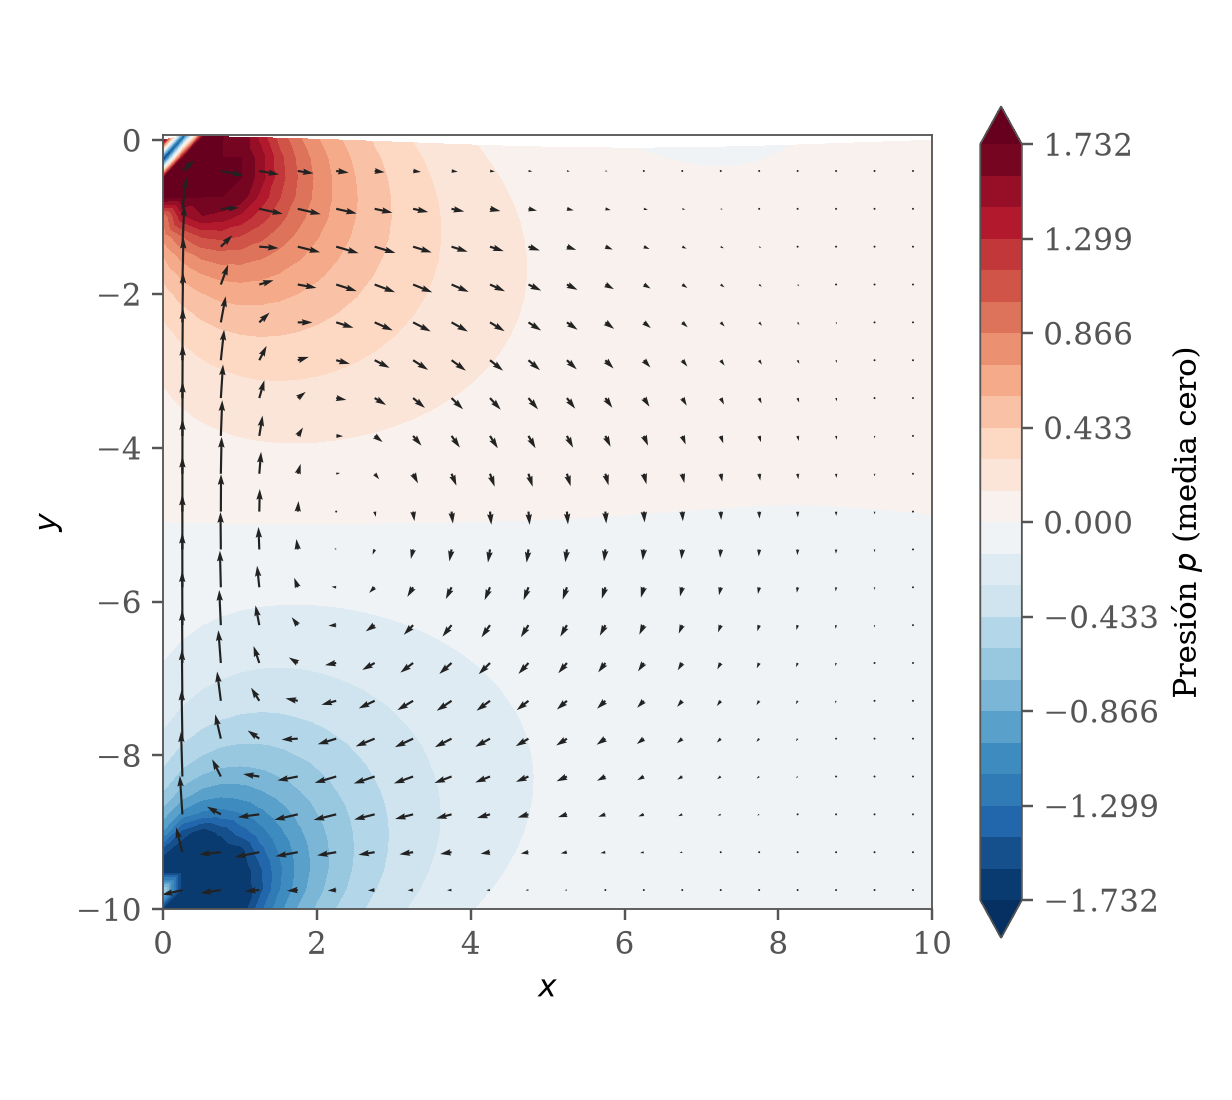
\includegraphics[width=0.75\textwidth]{../imagenes/FSI_velocidad_presion.png}
    \caption{Campo de velocidad (vectores) y distribución de presión de media cero (mapa de color) en el dominio deformado $\Omega_f$, malla $N = 40$. La escala de color se recorta a $|p| \le 1.73$ (percentil 98); los valores mayores se concentran en las esquinas de la pared impulsora.}
    \label{fig:velpre}
\end{figure}

\subsection{Respuesta estructural}

La deformación de la viga se visualiza en la Figura \ref{fig:de}. Sobre la interfaz, la tracción transmitida es $\alpha\,\boldsymbol{\sigma}_f \cdot \mathbf{n}_s$ con $\mathbf{n}_s = (0, -1)$, de modo que la presión positiva del fluido empuja la viga hacia arriba, en contra del peso propio. Como la presión es mayor cerca de la pared impulsora, ese empuje alivia la parte izquierda de la viga y la elástica resulta asimétrica: el desplazamiento vertical máximo, $|d_y| \approx 0.103$, se alcanza en $x \approx 6$ y no en el centro del vano, que es donde lo tendría una viga cargada solo por su peso. Junto al extremo izquierdo empotrado se observa además una deformación local hacia arriba ($d_y \approx 0.068$ en $x = 0.25$ para $N = 40$), producida por la presión singular de la esquina. Esta deformación queda confinada al primer elemento contiguo a la esquina y se desplaza hacia ella al refinar la malla ($d_y \approx 0.062$ en $x \approx 0.08$ para $N = 120$), lo que indica que es un efecto de la singularidad y no un rasgo de la respuesta global de la viga. En todos los casos los desplazamientos son del orden del 5\,\% del espesor de la viga, dentro del régimen de pequeñas deformaciones de la elasticidad lineal.

\begin{figure}[H]
    \centering
    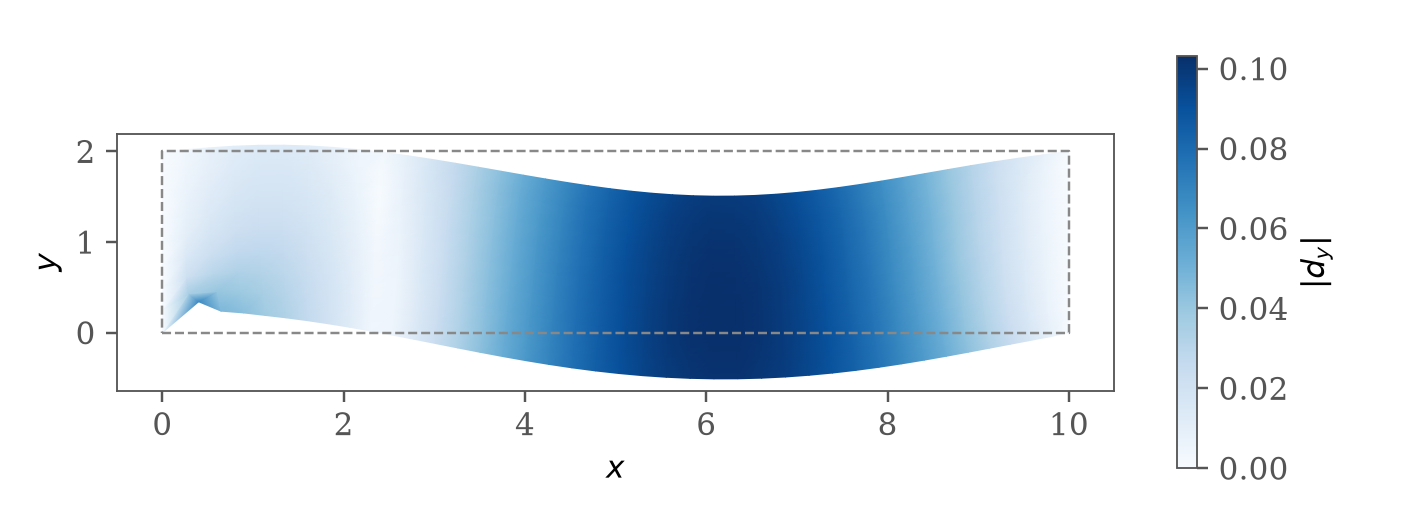
\includegraphics[width=0.85\textwidth]{../imagenes/FSI_desplazamiento_viga.png}
    \caption{Magnitud del desplazamiento vertical $|d_y|$ de la viga, malla $N = 40$. La geometría deformada se dibuja con los desplazamientos amplificados 5 veces; la línea discontinua indica la configuración de referencia.}
    \label{fig:de}
\end{figure}

\subsection{Adaptación de la malla (ALE)}

La Figura \ref{fig:movema} muestra la malla del fluido deformada cerca de la interfaz. La extensión armónica redistribuye los nodos internos de forma suave y la deformación se atenúa rápidamente hacia el interior de la cavidad. La condición $J_K > 0$ se comprobó numéricamente sobre la totalidad del dominio: se calculó, para cada triángulo, el cociente entre su área con signo en la malla deformada y su área en la malla de referencia. El valor mínimo de ese cociente es $0.962$ para $N = 40$ y $0.945$ para $N = 120$, de modo que ningún elemento se invierte ni se degenera.

\begin{figure}[H]
    \centering
    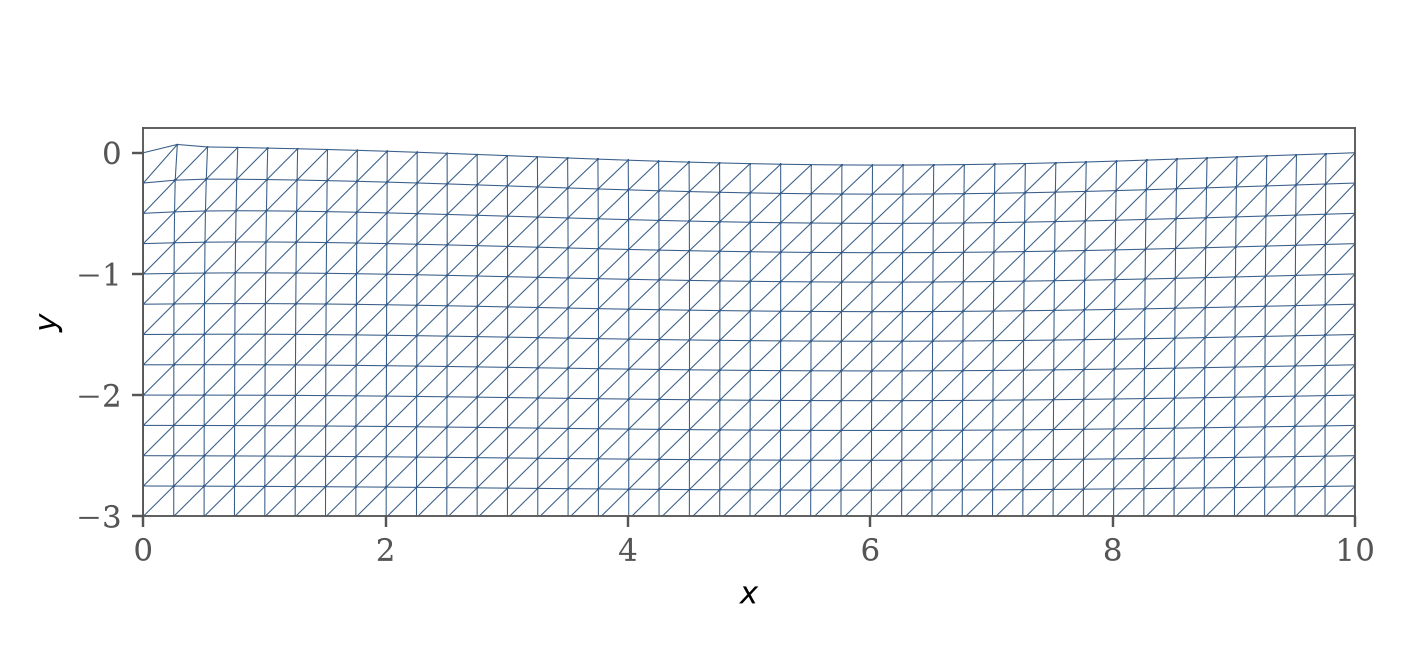
\includegraphics[width=0.85\textwidth]{../imagenes/FSI_malla_deformada.png}
    \caption{Malla del fluido deformada en la franja superior de la cavidad ($-3 \le y \le 0$), malla $N = 40$, sin amplificación.}
    \label{fig:movema}
\end{figure}

\section{Validación numérica: análisis de convergencia}

Ante la ausencia de una solución analítica cerrada para este problema no lineal de interacción fluido-estructura con frontera móvil, la validación del código se lleva a cabo mediante un estudio de convergencia de malla (\textit{Mesh Convergence Study}).

El objetivo principal es verificar numéricamente la consistencia del esquema, comprobando que el error de discretización disminuye conforme se refina la malla y estimando experimentalmente la tasa con que lo hace, para contrastarla con las estimaciones teóricas de los espacios de elementos finitos empleados.

\subsection{Metodología: solución de referencia}

Se ha generado una \textit{solución de referencia} $(\mathbf{u}_{\text{ref}}, p_{\text{ref}}, \mathbf{d}_{\text{ref}})$ utilizando una malla estructurada de alta densidad con $N=120$ subdivisiones por lado en la cavidad ($28\,800$ triángulos en el fluido). Se asume que esta solución sobre-refinada es una aproximación suficiente de la solución exacta del continuo.

Posteriormente, se resuelve el problema en una secuencia de mallas estructuradas más gruesas con $N \in \{10, 20, 40, 80\}$, en las que $h$ se divide exactamente a la mitad de una malla a la siguiente; la viga se discretiza con $N$ subdivisiones a lo largo y $\max(2, N/5)$ a través del espesor, de modo que los nodos de la interfaz coinciden en ambos subdominios. Dado que cada solución está definida sobre su propio dominio deformado, la comparación se hace a través de la configuración de referencia: la velocidad de referencia, expresada en la malla de referencia, se interpola en los nodos de la malla de referencia de nivel $N$, y la integral del error se evalúa sobre el dominio deformado de la malla $N$. El error se cuantifica proyectando la solución de referencia sobre el espacio de la malla gruesa y evaluando la norma $L^2$ del error relativo de la velocidad:

\begin{equation}
    E_N = \frac{\| \mathbf{u}_N - \mathcal{I}_N(\mathbf{u}_{\text{ref}}) \|_{L^2(\Omega_f)}}{\| \mathcal{I}_N(\mathbf{u}_{\text{ref}}) \|_{L^2(\Omega_f)}},
\end{equation}
donde $\mathcal{I}_N$ denota el operador de interpolación sobre los nodos de la malla actual $N$. En lo que sigue, el tamaño de malla se expresa en forma relativa, $h/L = 1/N$, con respecto a la longitud $L = 10$ del lado de la cavidad; dado que la tasa de convergencia depende únicamente de los cocientes entre pasos sucesivos, esta normalización no altera los órdenes estimados.

\subsection{Tasa de convergencia observada}

La Tabla \ref{tab:convergencia} resume la evolución del error. La tasa de convergencia experimental (orden estimado $q$) se calcula logarítmicamente entre mallas sucesivas:
\[
q = \frac{\log(E_{N-1} / E_N)}{\log(h_{N-1} / h_N)}.
\]

\begin{table}[H]
\centering
\renewcommand{\arraystretch}{1.2}
\small
\begin{tabular}{|c|c|c|c|c|}
    \hline
    \textbf{$N$} & \textbf{Paso relativo ($h/L$)} & \textbf{Error relativo $L^2$} & \textbf{Orden $q$} & \textbf{Deflexión máx.} \\ \hline
    10 & $1.00 \times 10^{-1}$ & $8.806 \times 10^{-2}$ & - & $0.0685$ \\ \hline
    20 & $5.00 \times 10^{-2}$ & $4.408 \times 10^{-2}$ & \textbf{1.00} & $0.0926$ \\ \hline
    40 & $2.50 \times 10^{-2}$ & $2.167 \times 10^{-2}$ & \textbf{1.02} & $0.1032$ \\ \hline
    80 & $1.25 \times 10^{-2}$ & $1.140 \times 10^{-2}$ & \textbf{0.93} & $0.1066$ \\ \hline
    120 (ref.) & $8.33 \times 10^{-3}$ & - & - & $0.1075$ \\ \hline
\end{tabular}
\caption{Análisis de convergencia de malla ($h$-refinement) para la velocidad. La última columna es el desplazamiento vertical máximo de la viga.}
\label{tab:convergencia}
\end{table}

Los resultados evidencian que el error se reduce aproximadamente por un factor de 2 al dividir $h$ a la mitad, es decir, una tasa de convergencia experimental aproximadamente lineal ($O(h)$). La deflexión máxima de la viga también se estabiliza al refinar: entre $N = 80$ y la referencia cambia menos del 1\,\%.

\begin{nota}
	Los elementos de fluido $P_2$ permiten teóricamente un orden $O(h^3)$ en norma $L^2$, pero las estimaciones del Capítulo \ref{chap:teoria} lo garantizan solo si la solución es suficientemente regular, $\mathbf{u} \in [H^3(\Omega_f)]^2$. El caso de estudio no cumple esa hipótesis. En las esquinas $(0, 0)$ y $(0, -L)$ la velocidad prescrita $(0, U_0)$ de la pared impulsora se encuentra con la condición $\mathbf{u} = \mathbf{0}$ de las paredes contiguas, de modo que el dato de Dirichlet es discontinuo. Una función con un salto no pertenece a $H^{1/2}(\partial\Omega_f)$, por lo que no admite un levantamiento en $H^1(\Omega_f)$ y la solución continua no tiene la regularidad que suponen las estimaciones: es la situación clásica de la cavidad impulsada, en la que la presión crece como $1/r$ cerca de las esquinas. En el problema discreto, la condición de borde se impone en los nodos y el salto queda repartido sobre un único elemento, de modo que la discontinuidad se resuelve solo al ritmo con que se refina la malla. Como interpretación numérica de estos resultados, el orden 1 observado parece estar gobernado por esa pérdida de regularidad, que domina sobre las demás fuentes de error (la aproximación geométrica de la interfaz deformada y la proyección $L^2$ de las tensiones) y no permite observarlas por separado en este estudio. El último orden ($0.93$) debe leerse con cautela, porque la malla $N = 80$ está relativamente cerca de la referencia $N = 120$.
\end{nota}

\subsection{Verificación gráfica}

La Figura \ref{fig:loglog} ilustra la convergencia en escala logarítmica. La pendiente de la curva numérica es aproximadamente paralela a la recta de referencia $O(h)$.

\begin{figure}[H]
\centering
\begin{tikzpicture}
    \begin{loglogaxis}[
        width=10cm, height=8cm,
        xlabel={Tamaño relativo de malla $h/L$},
        ylabel={Error Relativo $\|\mathbf{u} - \mathbf{u}_{\text{ref}}\|_{L^2}$},
        grid=both,
        grid style={line width=.1pt, draw=gray!20},
        major grid style={line width=.2pt,draw=gray!50},
        legend pos=north west,
        title={Curva de Convergencia del Esquema FSI},
        cycle list name=color list
        ]
        
        % Datos Numéricos
        \addplot+[
        mark=square*,
        line width=1.2pt,
        mark size=2.5pt,
        color=blue
        ]
        coordinates {
            (0.1, 0.08806)
            (0.05, 0.04408)
            (0.025, 0.02167)
            (0.0125, 0.01140)
        };
        \addlegendentry{Simulación FSI}

        % Línea de Referencia O(h)
        \addplot [
        color=red,
        dashed,
        line width=1pt,
        domain=0.01:0.12
        ]
        {0.88*x};
        \addlegendentry{Referencia $O(h)$}

        % Triángulo de Pendiente (Slope Triangle)
        \coordinate (A) at (axis cs: 0.03, 0.0125); % Punto ancla
        \coordinate (B) at (axis cs: 0.06, 0.0125); % Derecha
        \coordinate (C) at (axis cs: 0.06, 0.0250); % Arriba (2 veces mayor para orden 1)

        \draw[black, thick] (A) -- (B) node[midway, below] {\footnotesize 1};
        \draw[black, thick] (B) -- (C) node[midway, right] {\footnotesize 1};
        \draw[black, thick] (A) -- (C);

    \end{loglogaxis}
\end{tikzpicture}
\caption{Gráfico Log-Log del error relativo. El triángulo indica la pendiente $m=1$; los resultados numéricos evidencian una tasa de convergencia experimental aproximadamente lineal.}
\label{fig:loglog}
\end{figure}

En conclusión, los resultados indican que la implementación numérica es consistente y estable: el error disminuye de forma sistemática al refinar la malla y el acoplamiento converge en todos los niveles. El error relativo de la velocidad respecto de la solución de referencia es del 2.2\,\% para $N = 40$ y del 1.1\,\% para $N = 80$. La tasa observada es menor que la óptima de los elementos $P_2$, lo cual no indica un defecto de la implementación sino la falta de regularidad de la solución del caso de estudio; comprobar si se recupera un orden mayor al regularizar el dato de la pared impulsora, o al refinar la malla localmente en las esquinas, queda como trabajo futuro.

% CAPÍTULO 4: CONCLUSIONES
\chapter{Conclusiones y trabajo futuro}

\section{Discusión: alcances y limitaciones del modelo}

Los resultados numéricos presentados en el capítulo anterior muestran que el código desarrollado resuelve de forma consistente el problema acoplado en el caso de estudio: el acoplamiento converge, la malla deformada se mantiene válida y el error disminuye al refinar la malla. Se trata de una verificación frente a una solución de referencia propia, no de una validación frente a datos experimentales o soluciones de la literatura; además, la tasa de convergencia observada está limitada por la falta de regularidad del caso, de modo que no permite contrastar cuantitativamente las estimaciones óptimas del Capítulo \ref{chap:teoria}. Sin embargo, para una interpretación rigurosa de estos hallazgos, es fundamental analizar críticamente el rango de validez de las hipótesis físicas adoptadas y las restricciones inherentes a la estrategia numérica.

\subsection{Validez del modelo físico}

El presente trabajo se ha circunscrito al régimen de flujo de Stokes y elasticidad lineal. Estas simplificaciones, aunque necesarias para un primer abordaje, conllevan limitaciones específicas:

\begin{itemize}
    \item \textbf{Desprecio de efectos inerciales:} La omisión del término convectivo no lineal $(\mathbf{u} \cdot \nabla)\mathbf{u}$ en las ecuaciones del fluido restringe la validez del modelo a números de Reynolds muy bajos ($Re \ll 1$). En aplicaciones con fluidos de baja viscosidad (como agua o aire) o altas velocidades, la inercia jugaría un papel determinante en la dinámica de la viga, pudiendo inducir inestabilidades aeroelásticas (como el \textit{flutter}) que este modelo cuasi-estático no puede capturar.
    
    \item \textbf{Hipótesis de linealidad geométrica y material:} Aunque el método ALE permite gestionar el movimiento de la frontera, la ley constitutiva del sólido se mantiene bajo la hipótesis de elasticidad lineal (pequeñas deformaciones). Si las fuerzas hidrodinámicas provocaran una deflexión en la tapa superior comparable a su espesor o longitud ($|\mathbf{d}| \sim L$), se violarían las hipótesis de la teoría lineal. En tal escenario, sería imperativo adoptar modelos hiperelásticos (e.g., Neo-Hookean o Mooney-Rivlin) y una formulación Lagrangiana Total o Actualizada para describir correctamente el estado tensional.
\end{itemize}

\subsection{Estabilidad del esquema particionado}

La estrategia de acoplamiento segregado (Dirichlet-Neumann) con relajación constante resultó efectiva para el caso de prueba estudiado. No obstante, la literatura especializada advierte que este enfoque es susceptible al ``efecto de masa añadida'' (\textit{added-mass effect}) \cite{causin2005added}.

Cuando la densidad del fluido es comparable a la del sólido ($\rho_f \approx \rho_s$), el operador de iteración de punto fijo se vuelve numéricamente inestable. Esto obliga a utilizar factores de relajación extremadamente pequeños ($\omega \to 0$), lo que incrementa drásticamente el costo computacional. En este trabajo, la convergencia fue rápida debido a la alta viscosidad del fluido y la rigidez relativa de la estructura, pero la robustez del algoritmo podría degradarse severamente en configuraciones con estructuras más ligeras o flexibles.

\subsection{Límites de la técnica ALE}

El método \textit{Arbitrary Lagrangian-Eulerian} (ALE) preserva la topología de la malla, deformando los elementos internos como una red elástica ficticia. Existe, sin embargo, un límite geométrico insalvable: si el desplazamiento de la frontera es excesivo, los elementos finitos (triángulos) del dominio fluido pueden sufrir distorsiones severas o incluso invertirse (Jacobiano $J_K \le 0$), provocando el fallo inmediato del solver.

Si bien la malla resistió las deformaciones moderadas del caso de estudio, para escenarios que involucren grandes rotaciones o contacto estructural, sería necesario transicionar hacia formulaciones ALE estabilizadas o técnicas de remallado adaptativo \cite{gao2025stabilized}, esquemas de acoplamiento con métodos de partículas \cite{yao2023improved}, o métodos de frontera inmersa (\textit{Immersed Boundary Methods}) \cite{kolahdouz2023sharp, wang2025three}, los cuales evitan la degradación de la calidad de la malla a costa de una mayor complejidad en la definición de la interfaz.

\section{Conclusiones}

En este trabajo de grado se ha descrito, modelado y simulado numéricamente un problema de interacción fluido-estructura (FSI) utilizando el Método de los Elementos Finitos (MEF). A partir del desarrollo teórico y los resultados obtenidos mediante el software FreeFEM++, se derivan las siguientes conclusiones:

\begin{enumerate}
    \item \textbf{Viabilidad del esquema particionado:} La implementación de un algoritmo segregado de tipo Dirichlet-Neumann permitió acoplar exitosamente las físicas del fluido (Stokes) y del sólido (Elasticidad Lineal). Se verificó, para el caso estudiado, que un enfoque iterativo es suficiente para resolver el acoplamiento en régimen estacionario: converge en 21 iteraciones con $\omega = 0.5$ y en 5 a 7 sin relajación, debido al carácter débil del acoplamiento, permitiendo la reutilización de solucionadores modulares sin la complejidad computacional de un sistema monolítico.
    
    \item \textbf{Estabilidad numérica y condición LBB:} Se verificó la importancia crítica de satisfacer la condición \textit{inf-sup} para el problema del fluido. El uso del par estable de Taylor-Hood ($P2/P1$) garantizó la estabilidad del campo de presión frente a modos espurios; sin embargo, cabe precisar que la estabilidad de este par no garantiza, por sí sola, la precisión absoluta de las fuerzas de tracción proyectadas sobre la interfaz, lo cual sigue siendo un desafío inherente a los esquemas particionados.
    
    \item \textbf{Robustez de la formulación ALE:} La técnica Arbitraria Lagrangiana-Euleriana demostró ser una herramienta robusta para gestionar la deformación del dominio fluido. El método de extensión armónica para el movimiento de la malla preservó la calidad de los elementos finitos en el rango de deflexiones considerado: el cociente mínimo entre el área deformada y el área de referencia de los triángulos fue $0.945$ en la malla más fina, sin elementos invertidos ni degenerados.

    \item \textbf{Coherencia física de los resultados:} La presión del fluido, mayor junto a la pared impulsora, alivia el lado izquierdo de la viga y produce una elástica asimétrica, con la deflexión máxima desplazada hacia $x \approx 6$. Se observó también que la respuesta estructural es sensible a los gradientes de presión locales, en particular a la singularidad de la esquina superior izquierda, lo que subraya la necesidad de un acoplamiento bidireccional preciso para modelar sistemas multifísicos reales.

    \item \textbf{Relación entre el análisis y la simulación:} El estudio de convergencia evidencia una tasa aproximadamente lineal en la velocidad, menor que la óptima de los elementos $P_2$. La diferencia se explica porque las estimaciones de error del Capítulo \ref{chap:teoria} suponen una regularidad que el caso de estudio no tiene, debido a la discontinuidad del dato de Dirichlet en las esquinas de la pared impulsora; el análisis teórico identifica así la causa de la tasa observada.
\end{enumerate}

\section{Trabajo futuro}
\label{sec:trabajo_futuro}

Para extender el alcance de este trabajo, se proponen los siguientes puntos:

\begin{itemize}
    \item \textbf{Extensión a Navier-Stokes:} Incorporar el término convectivo no lineal $(\mathbf{u} \cdot \nabla)\mathbf{u}$ para analizar el sistema a números de Reynolds moderados, donde los efectos inerciales y la formación de vórtices secundarios podrían alterar drásticamente la distribución de esfuerzos sobre la estructura.
    
    \item \textbf{Análisis en el dominio del tiempo:} Implementar esquemas de integración temporal (e.g., Newmark-$\beta$ o Euler implícito) para estudiar la respuesta dinámica del sistema, permitiendo la identificación de fenómenos de resonancia, amortiguamiento fluido-elástico o flameo (\textit{flutter}).
    
    \item \textbf{No-linealidad geométrica y material:} Sustituir el modelo de elasticidad lineal por una formulación de grandes desplazamientos basada en modelos hiperelásticos (como San Venant-Kirchhoff o Neo-Hookeano), lo cual permitiría simular con fidelidad materiales de baja rigidez como tejidos biológicos o elastómeros.
    
    \item \textbf{Aceleración del acoplamiento y movimiento de malla:} Reemplazar la relajación de parámetro constante por métodos de tipo cuasi-Newton, que aceleran la convergencia del lazo particionado sin requerir el ensamblaje del sistema monolítico \cite{delaisse2023quasinewton}, e incorporar extensiones ALE estabilizadas o marcos particionados recientes capaces de admitir desplazamientos de interfaz mayores que los alcanzables mediante la extensión armónica empleada en este trabajo \cite{gao2025stabilized, zhang2024efficient}.

    \item \textbf{Regularidad y validación cuantitativa:} Repetir el estudio de convergencia con un dato regularizado en la pared impulsora, que se anule en las esquinas, o con refinamiento local de la malla en ellas, para comprobar si se recupera el orden óptimo de los elementos $P_2$; recuperar la carga sobre la interfaz mediante el residuo variacional del fluido en lugar de la proyección $L^2$ de las tensiones; y contrastar los resultados con datos de referencia externos, como los de la cavidad impulsada \cite{ghia1982high}.
\end{itemize}

% --- BIBLIOGRAFIA ---
\printbibliography[heading=bibintoc]


% ==========================================================
%  ANEXO: CODIGO DE LA SIMULACION
% ==========================================================
\appendix
\chapter{Código de la simulación en FreeFEM++}
\label{anexo:codigo}

{\sloppy
Este anexo reproduce el programa con el que se obtuvieron todos los resultados del Capítulo \ref{chap:implementacion} (archivo \texttt{programas/FSI\_Particionado.edp}). Las figuras corresponden a la ejecución con las opciones \texttt{-N 40 -export 1}. El estudio de convergencia corresponde a una ejecución con \texttt{-N 120 -ref 1}, que guarda la solución de referencia, seguida de las ejecuciones con \texttt{-N} igual a 10, 20, 40 y 80 y la opción \texttt{-cmp 120}. La prueba sin relajación usa la opción \texttt{-omega 1}. Las figuras se dibujan a partir de los archivos exportados con el programa \texttt{programas/figuras\_FSI.py}.\par}

\lstinputlisting[caption={Programa completo del esquema particionado (\texttt{FSI\_Particionado.edp})}]{../programas/FSI_Particionado.edp}

\end{document}
